\documentclass[../main.tex]{subfiles}
\begin{document}
\newpage
\thispagestyle{empty}
\begin{center}
    {
\includegraphics[width=0.5\textwidth]{Imagenes/Logo UMA.jpg}\par}
    \vspace{1cm}
    {\bfseries\LARGE \Facultad \par}
    \vspace{0.5cm}
    {\scshape\Large \Grado \par}
    \vspace{1.5cm}
    {\scshape\Huge Anexo III \par}
    \vspace{1.5cm}
    {\scshape\Huge Diseño de Instalación de Iluminación \par}
    \vspace{0.5cm}
    {\itshape\Large \TituloProyecto \par}
    \vfill
    {\Large Solicitante: \par}
    {\Large \Solicitante  \par}
    \vspace{1cm}
    {\Large Autores: \par}
    {\Large \Autora \par}
    {\Large \Autor \par}
    \vfill
    {\Large \Fecha \par}
\end{center}

\newpage
\section{Introducción}
Para el diseño de la instalación de iluminación del proyecto, se ha utilizado el programa DIALux Evo 12.0, con el que se han realizado todos los cálculos. \par
\vspace{0.5 cm}
En este anexo se detallarán los cálculos y resultados obtenidos por dicha aplicación, así como las consideraciones que se han tenido en cuenta para cada estancia, como son la superficie, altura y actividad que se va a llevar a cabo en dicha estancia. \par
\vspace{0.5 cm}
A la hora de la realización de estos cálculos, se tienen en cuenta las diferentes alturas de las estancias que conforman la nave. Siendo todas ellas de 3 metros, exceptuando las alturas de la planta de producción y el almacén, que serán de 6 metros. \par
\vspace{0.5 cm}
Para cada estancia, se deberá cumplir lo indicado por la norma UNE 12464-1, también se tendrá en consideración aquello establecido en el documento básico de ahorro de energía, concretamente el HE3.

\section{Consideraciones para el cálculo de las luminarias}
Para el dimensionamiento de las luminarias se han tenido en cuenta las siguientes consideraciones:

\begin{itemize}
    \item Se tomarán el catálogo del fabricante Philips para la elección de las luminarias del edificio.
    \item Se utilizará el mínimo número de luminarias con el que se cumplan los requisitos.
    \item Para asegurar una correcta iluminación para cualquier luz externa, se tendrá en cuenta una iluminación externa nula.
    \item El factor de degradación global será de 0,8.
    \item Se toman unos coeficientes de reflexión estándar según la norma.
    \item La iluminancia media (Em) tendrá que ser mayor a la indicada en la norma.
    \item El índice de deslumbramiento unificado (UGR) máximo calculado deberá ser menor que el indicado por la normativa para el tipo de actividad que se realiza en la estancia.
    \item La uniformidad de la iluminancia (Uo) obtenida debe ser mayor a la dispuesta en la normativa.
    \item La reproducción cromática (Ra) mínima calculada deberá ser mayor que la indicada por la norma para dicha estancia.
    \item El valor de eficiencia energética de la instalación (VEII) no superará el valor límite establecido en la Tabla 3.1-HE3.
    \item La potencia total (Pmáx) de lámparas y equipos auxiliares por superficie iluminada no superará el valor máximo establecido en la Tabla 3.2-HE3.
\end{itemize}

\section{Parámetros de iluminación a cumplir según la estancia}
La nave cuenta de una planta baja en donde se encontrará el almacén, la planta de producción, una zona de exposición con oficina y baños de uso público y accesibles para minusválidos. Por último, en la entreplanta, encontraremos zonas de uso exclusivo para el personal como pueden ser los vestuarios y una zona de descanso.\par
\vspace{0.5 cm}
En la siguiente tabla se detallan las dimensiones de cada estancia con los parámetros de iluminación que deben cumplir debido a su actividad según la norma UNE 12464-1. 

\begin{table}[H]
    \centering
    \begin{tabular}{c | c | c | c | c | c | c | c }
         Estancia & Superficie (m2) & Em & UGR & Uo  & Ra & VEEI & Pmáx \\ \hline
         Planta de Producción & 620,0366 & 500 & 19 & 0,6 & 80 & 5,0 & 25 \\
         Baños & 10,5625 & 200 & 25 & 0,4 & 80 & 4,0 & 10 \\
         Baño Minusválidos & 6,82 & 200 & 25 & 0,4 & 80 & 4,0 & 10 \\
         Zona Exposición & 43,5431 & 300 & 22 & 0,4 & 80 & 4,0 & 10 \\
         Oficina & 10 & 500 & 19 & 0,6 & 80 & 3,0 & 10 \\
         Almacén & 111,3 & 100 & 25 & 0,4 & 60 & 4,0 & 10 \\
         Vestuarios & 20,3156 & 200 & 25 & 0,4 & 80 & 4,0 & 10 \\
         Zona Descanso & 41,4685 & 100 & 22 & 0,4 & 80 & 4,0 & 10 \\
    \end{tabular}
    \caption{Superficies y parámetros de iluminación de las estancias de la nave.}
\end{table}

\section{Resultados de la iluminación obtenida en DIALux}
\subsection{Luminarias empleadas}
\begin{figure}[H]
    \centering
    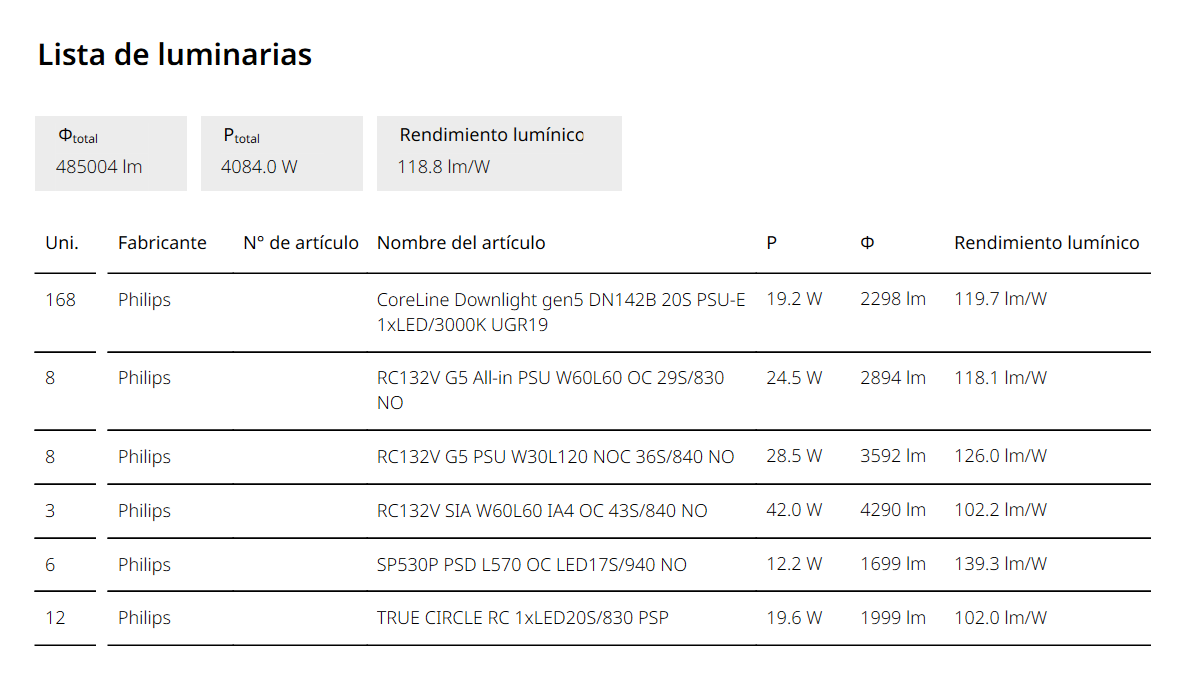
\includegraphics[width=0.75\linewidth]{Imagenes/Lista de luminarias.png}
    \caption{Luminaria empleada en la nave.}
\end{figure}

\subsection{Planta de Producción}
\begin{figure}[H]
    \centering
    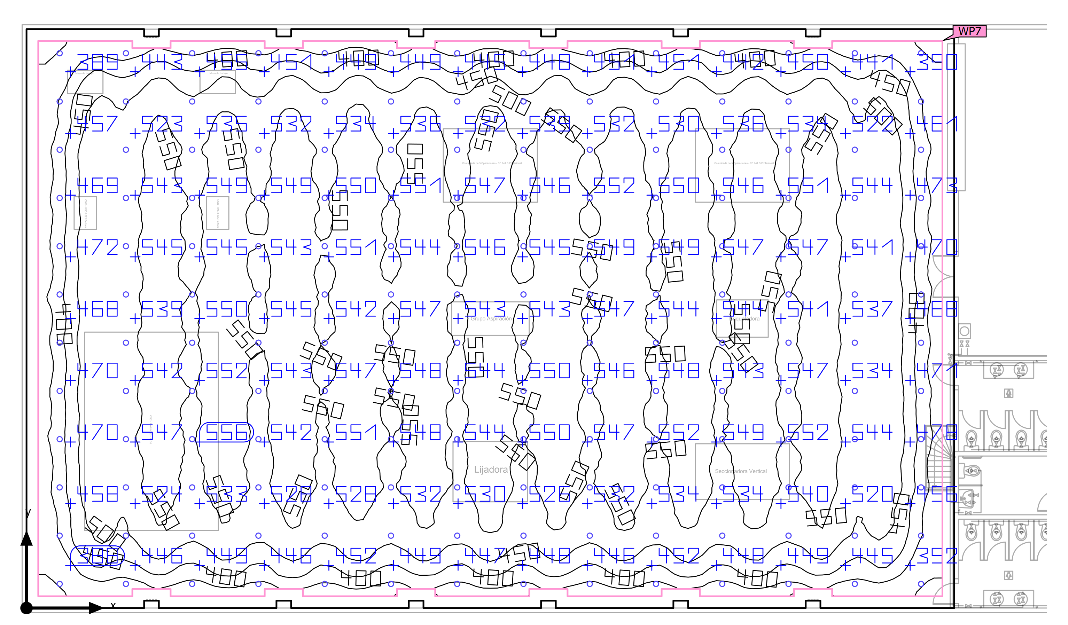
\includegraphics[width=0.5\linewidth]{Imagenes/Iluminacion Planta Produccion.png}
    \caption{Gráfico flujo luminoso en Planta de Producción.}
\end{figure}

\begin{figure}[H]
    \centering
    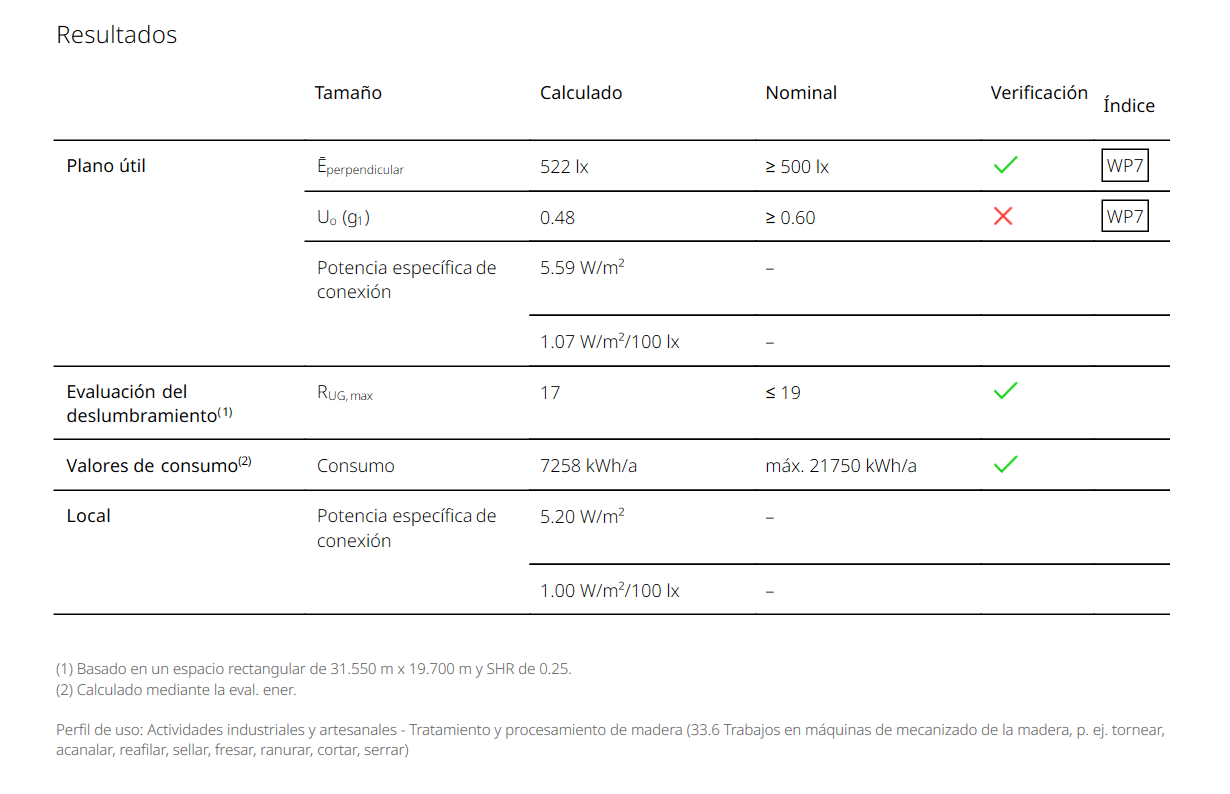
\includegraphics[width=0.75\linewidth]{Imagenes/Resultados Iluminacion Planta de Produccion.png}
    \caption{Resultados luminotécnicos Planta de Producción.}
\end{figure}

\subsection{Baño Femenino}
\begin{figure}[H]
    \centering
    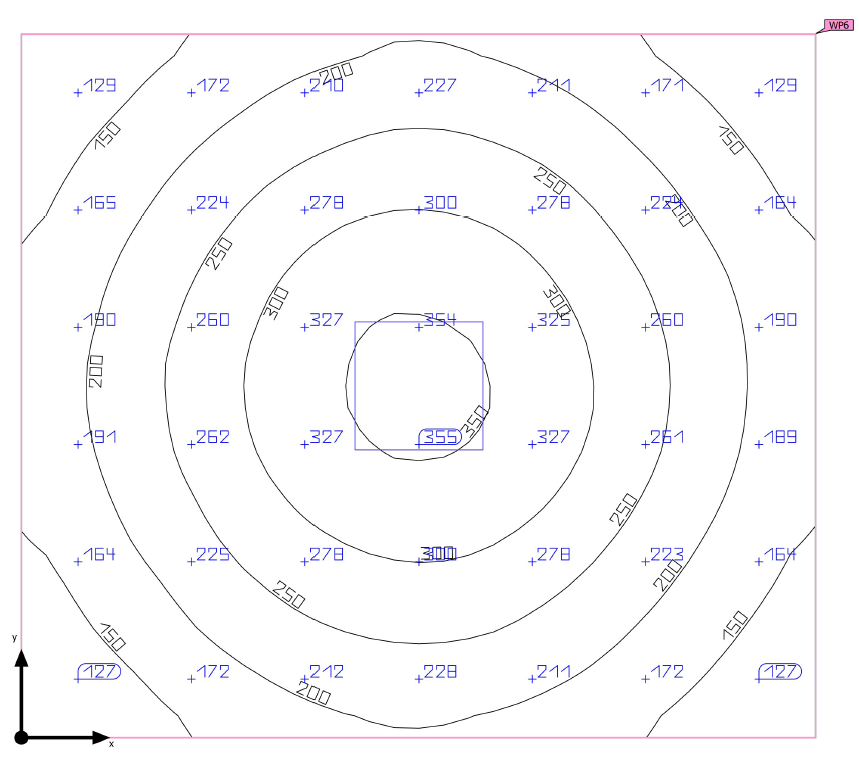
\includegraphics[width=0.5\linewidth]{Imagenes/Iluminacion Bano Femenino.png}
    \caption{Gráfico flujo luminoso en Baño Femenino.}
\end{figure}

\begin{figure}[H]
    \centering
    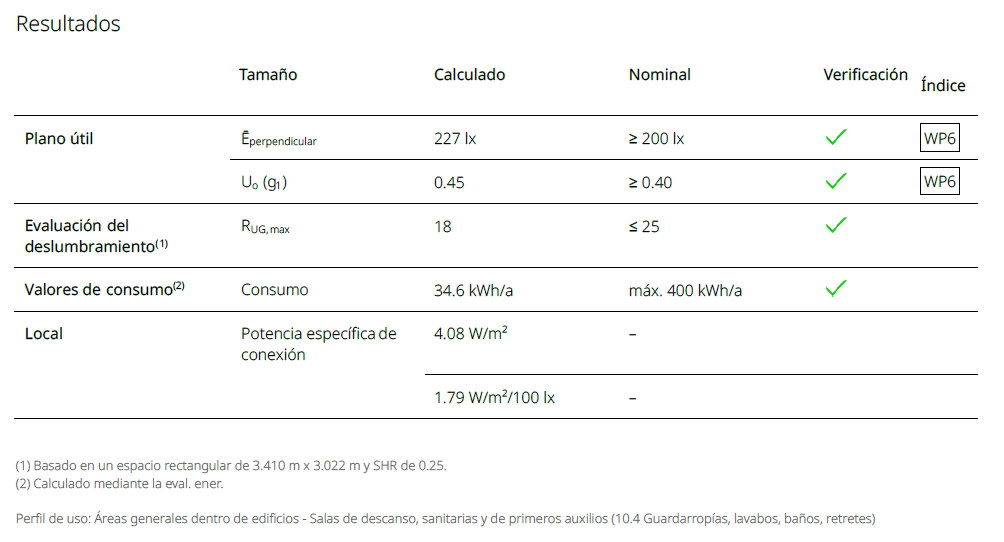
\includegraphics[width=0.75\linewidth]{Imagenes/Resultados Iluminacion Bano Femenino.png}
    \caption{Resultados luminotécnicos Baño Femenino.}
\end{figure}

\subsection{Baño Masculino}
\begin{figure}[H]
    \centering
    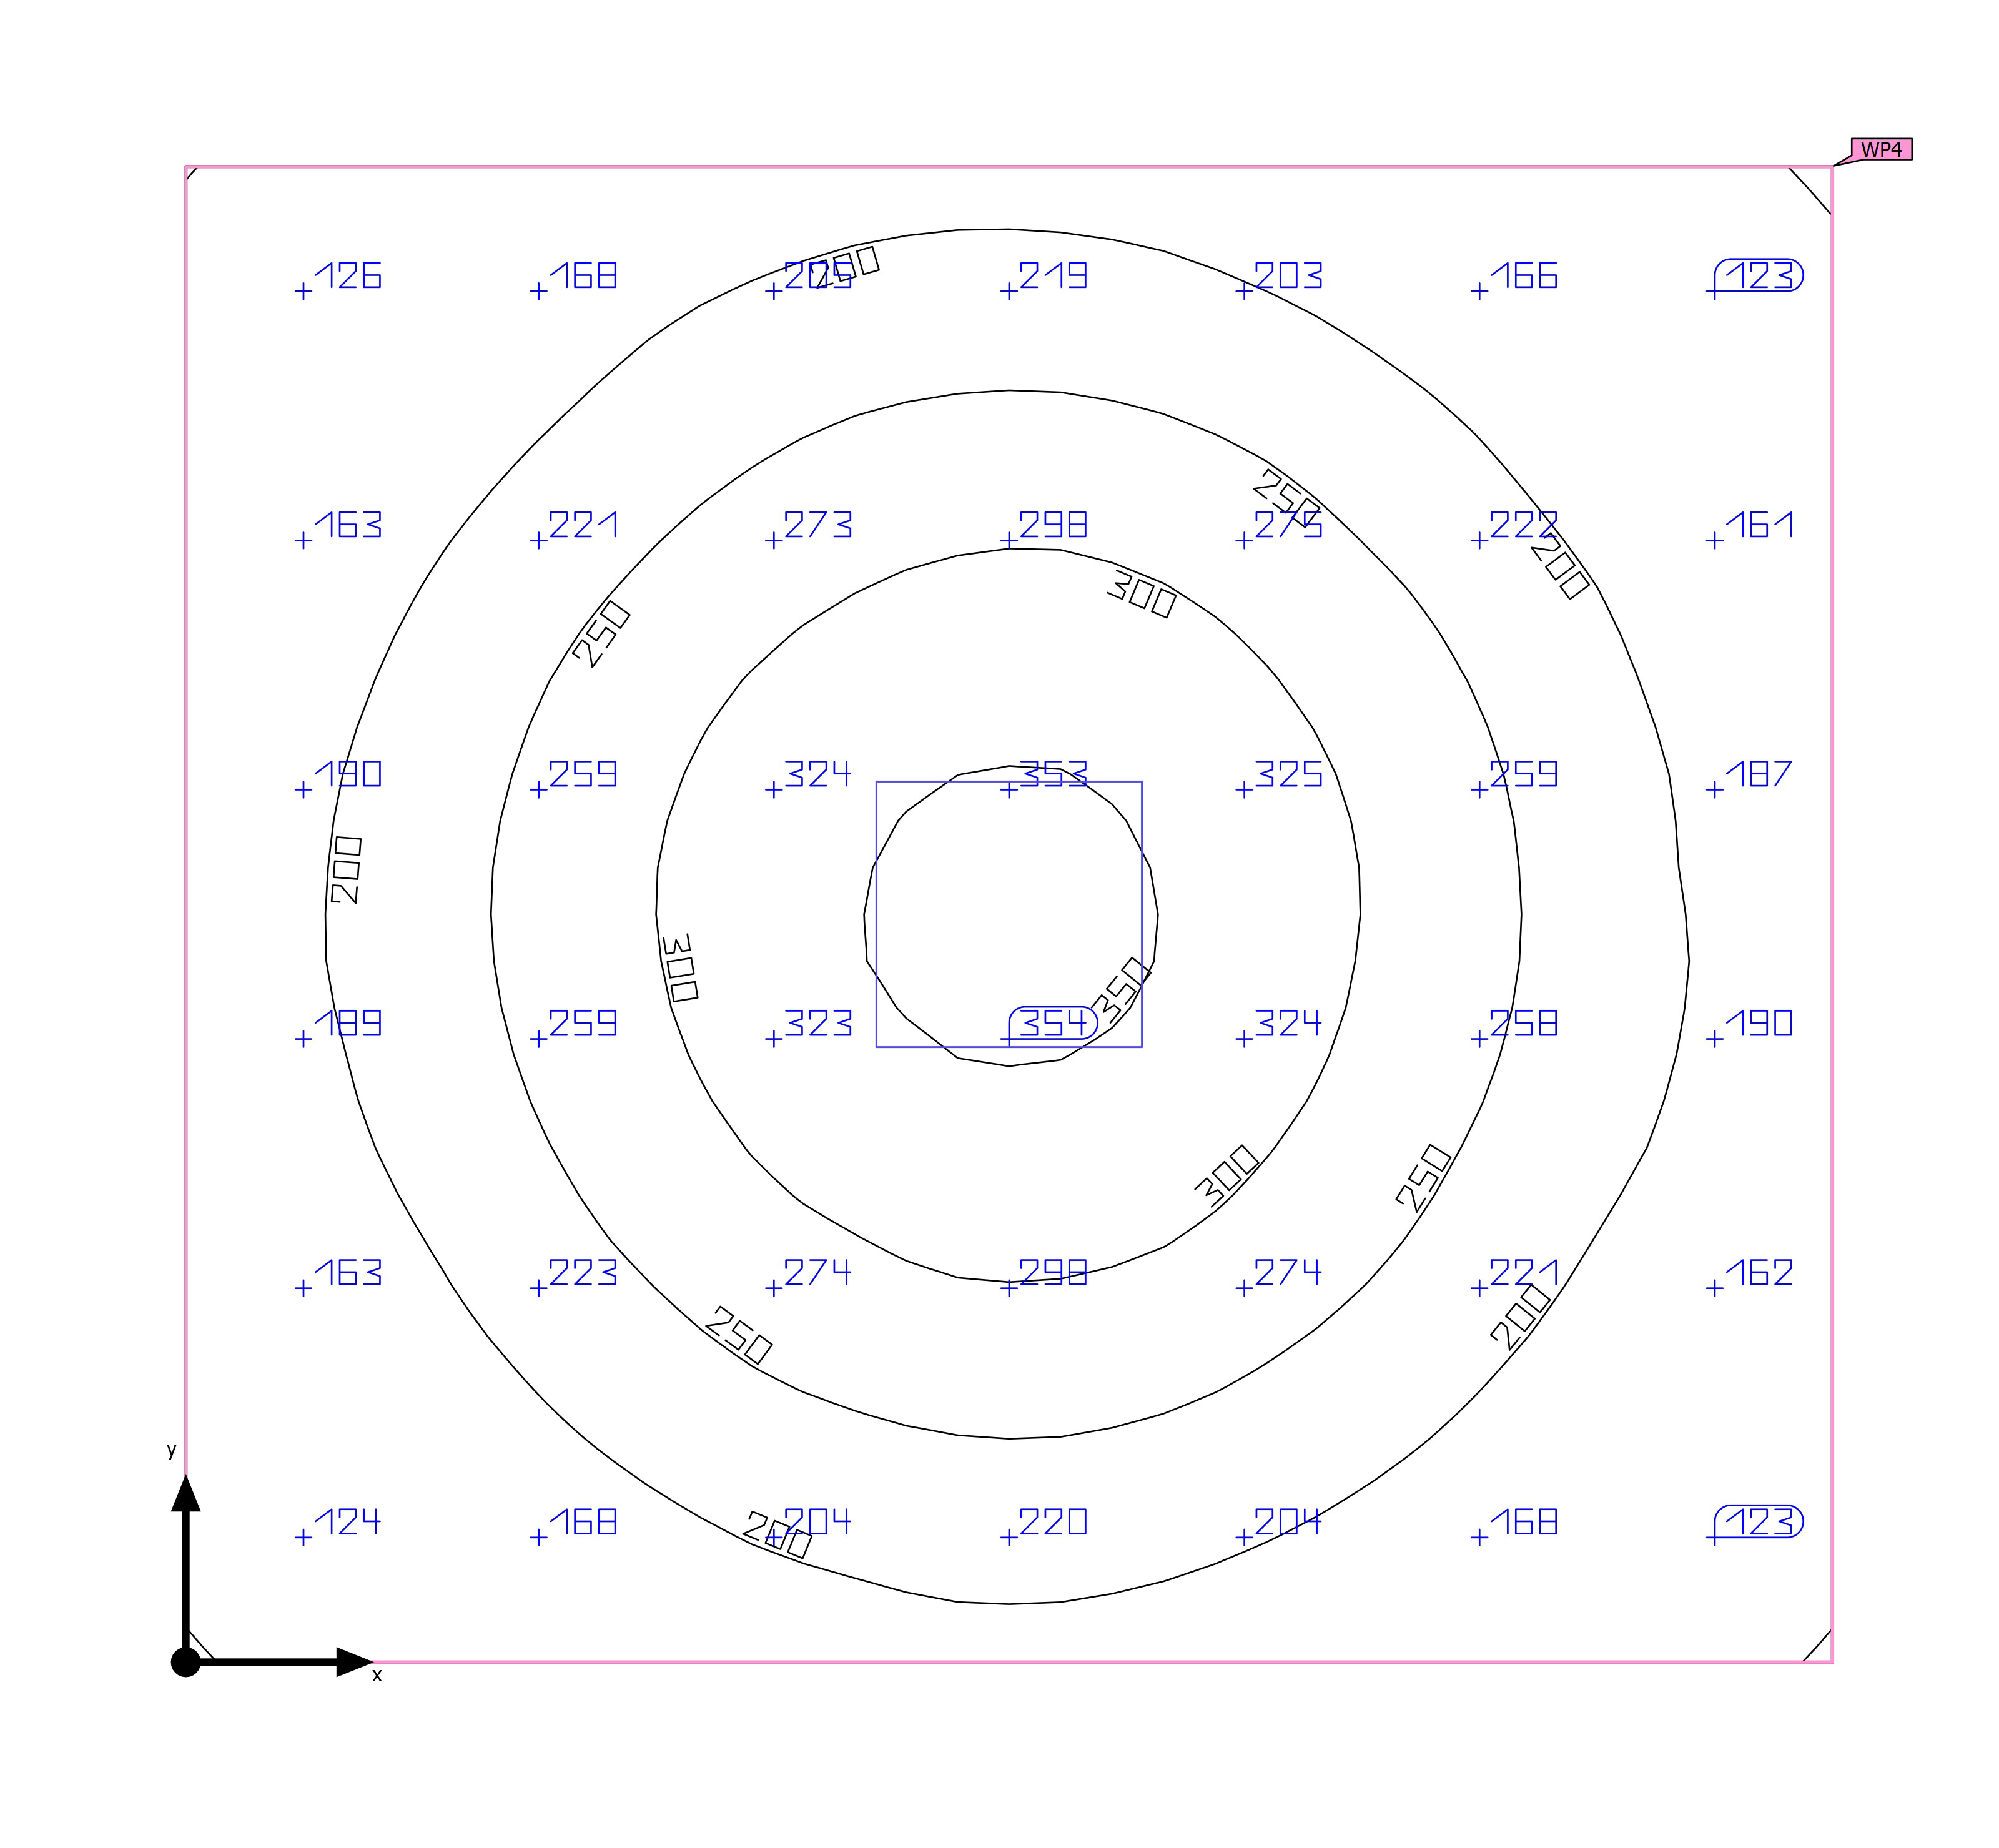
\includegraphics[width=0.5\linewidth]{Imagenes/Iluminacion Bano Masculino.png}
    \caption{Gráfico flujo luminoso en Baño Masculino.}
\end{figure}

\begin{figure}[H]
    \centering
    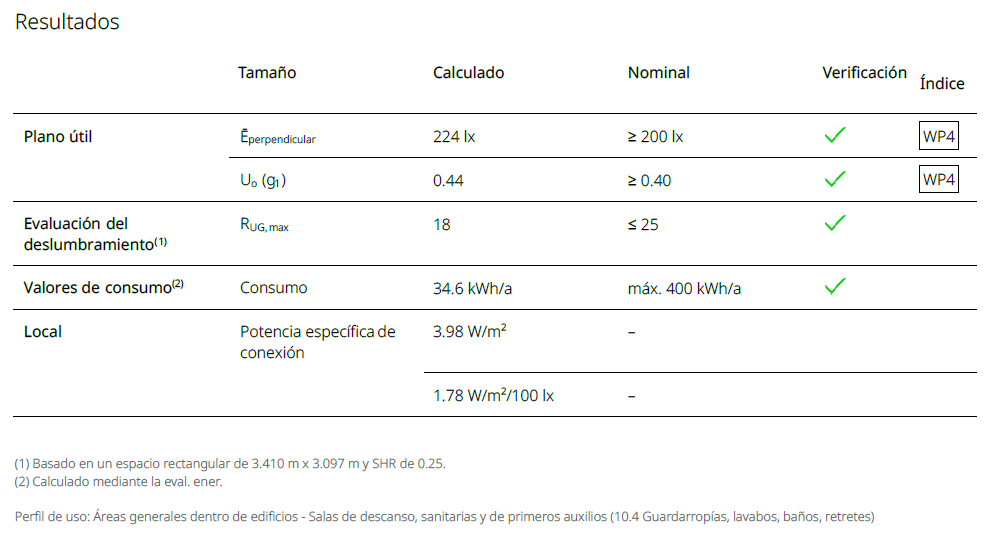
\includegraphics[width=0.75\linewidth]{Imagenes/Resultados Iluminacion Bano Masculino.png}
    \caption{Resultados luminotécnicos Baño Masculino.}
\end{figure}

\subsection{Baño Minusválidos}
\begin{figure}[H]
    \centering
    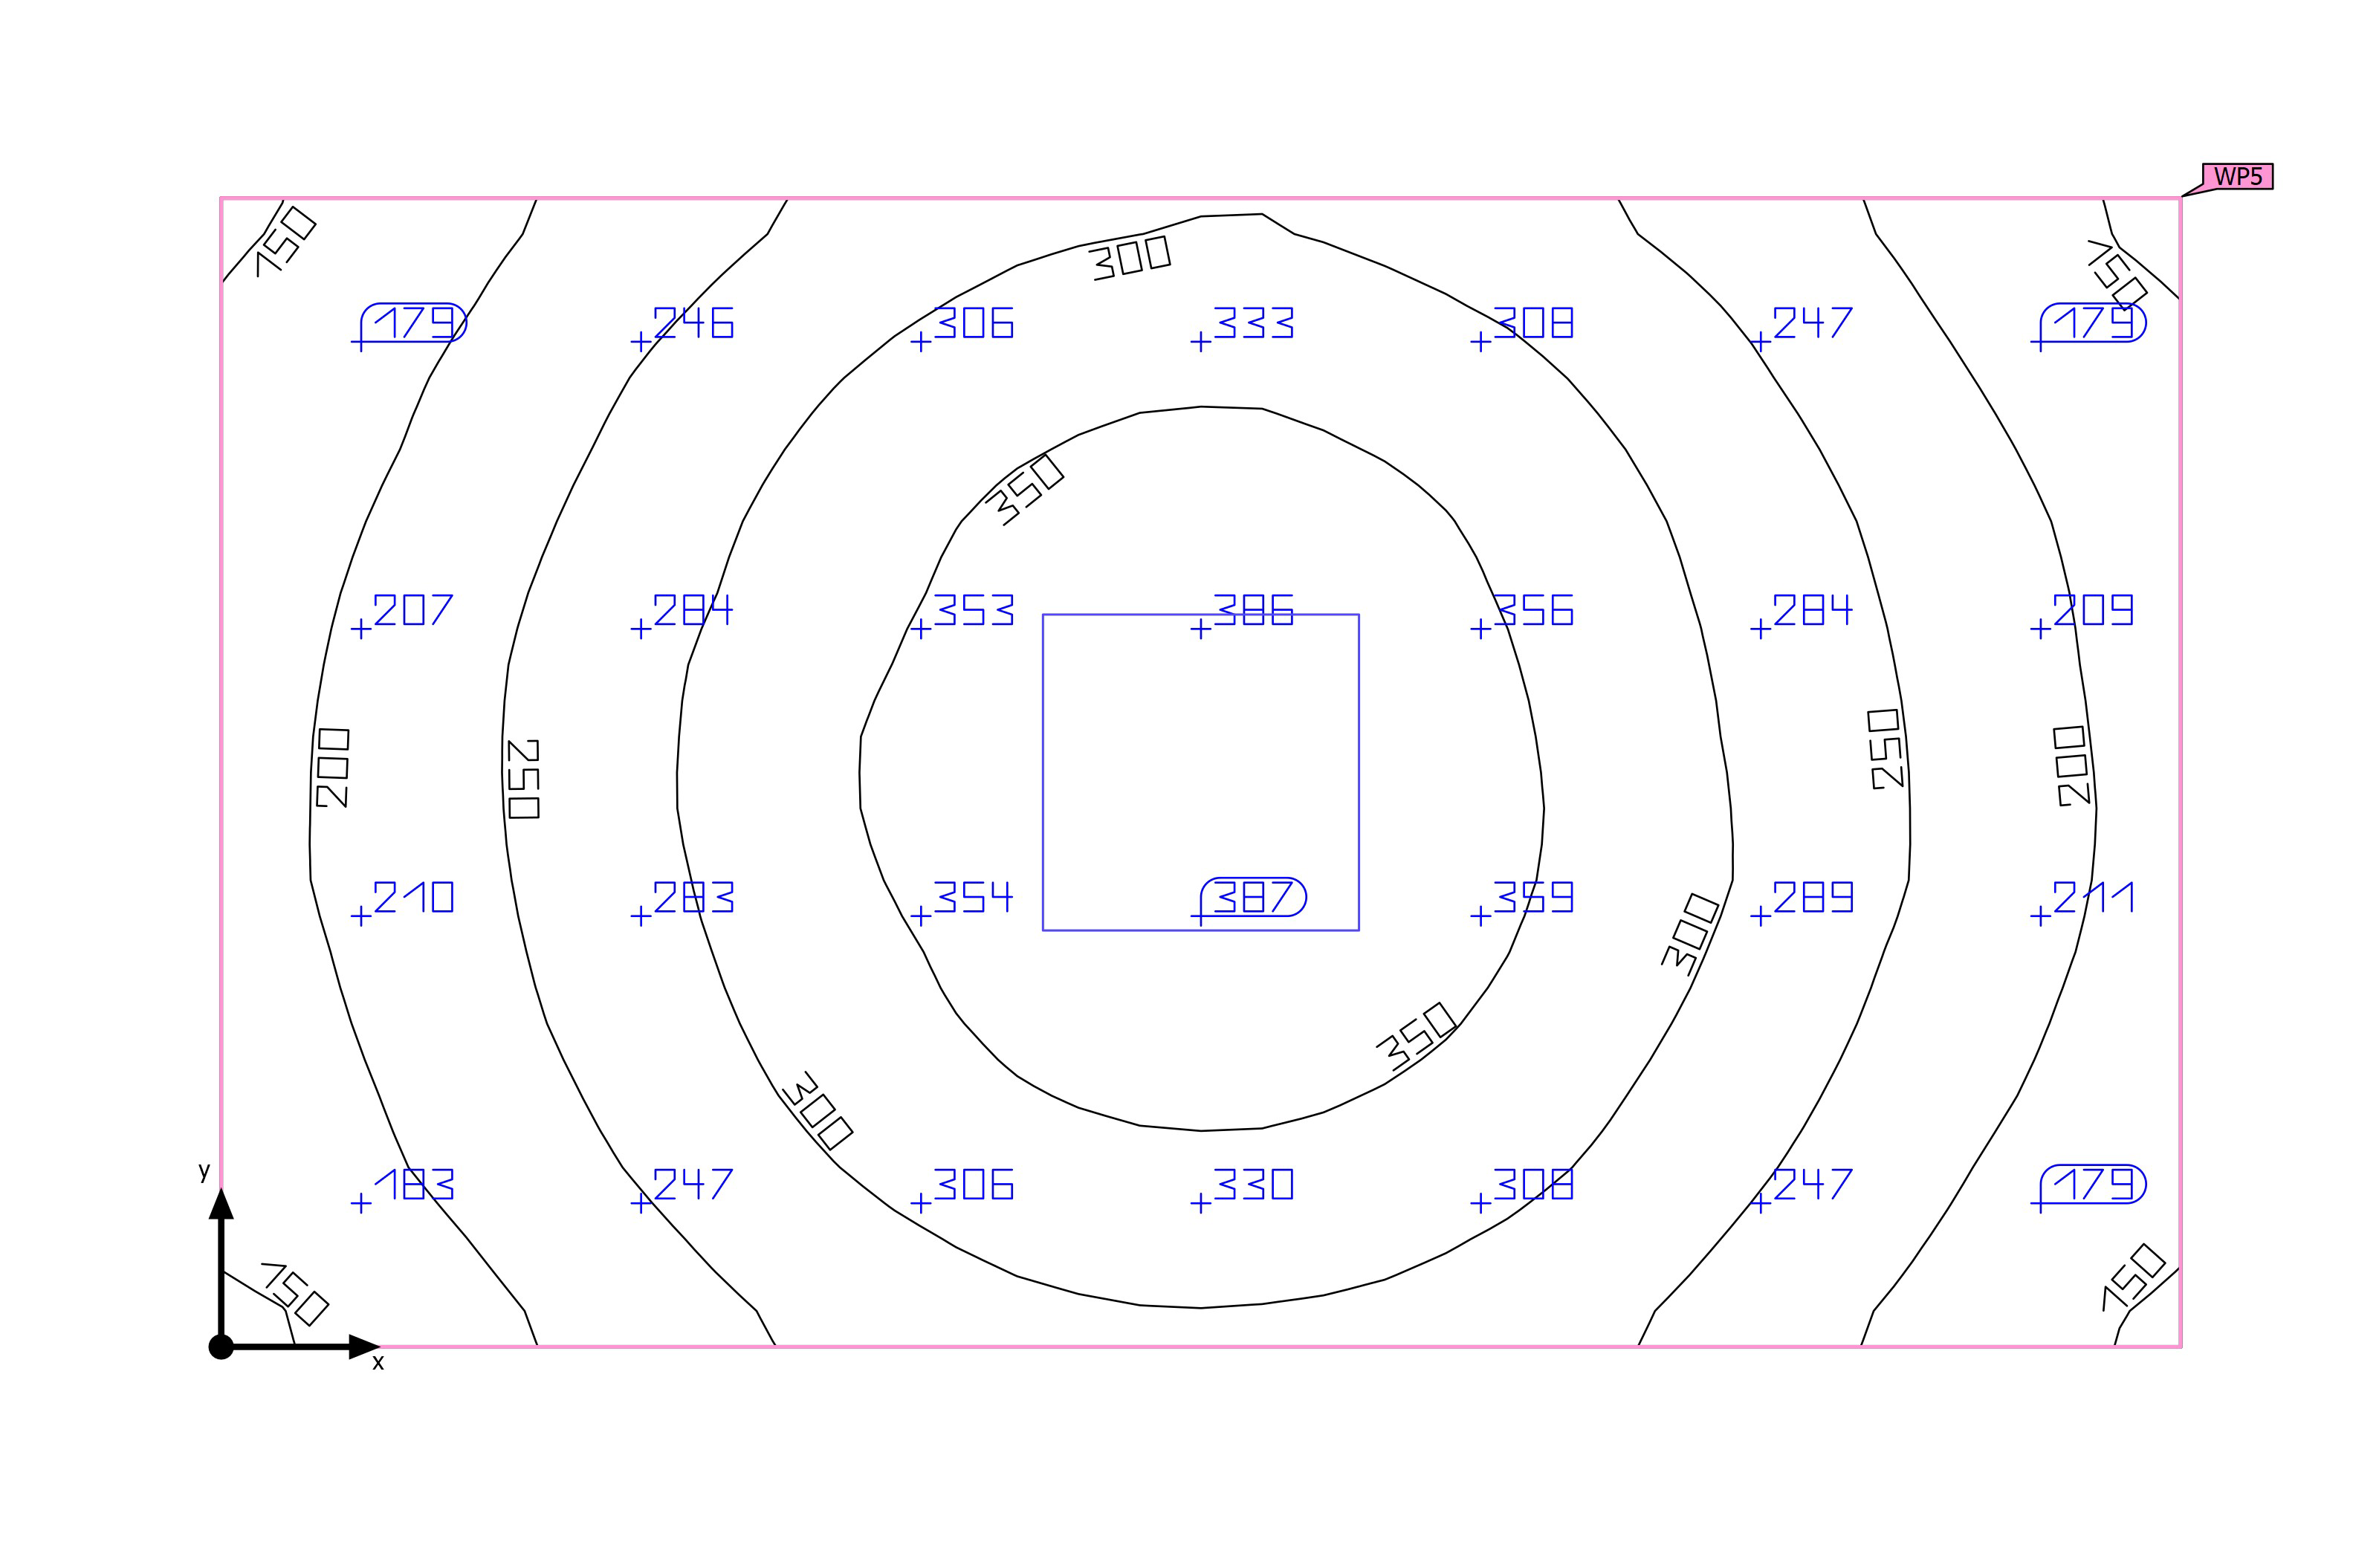
\includegraphics[width=0.5\linewidth]{Imagenes/Iluminacion Bano Minusvalidos.png}
    \caption{Gráfico flujo luminoso en Baño Minusválidos.}
\end{figure}

\begin{figure}[H]
    \centering
    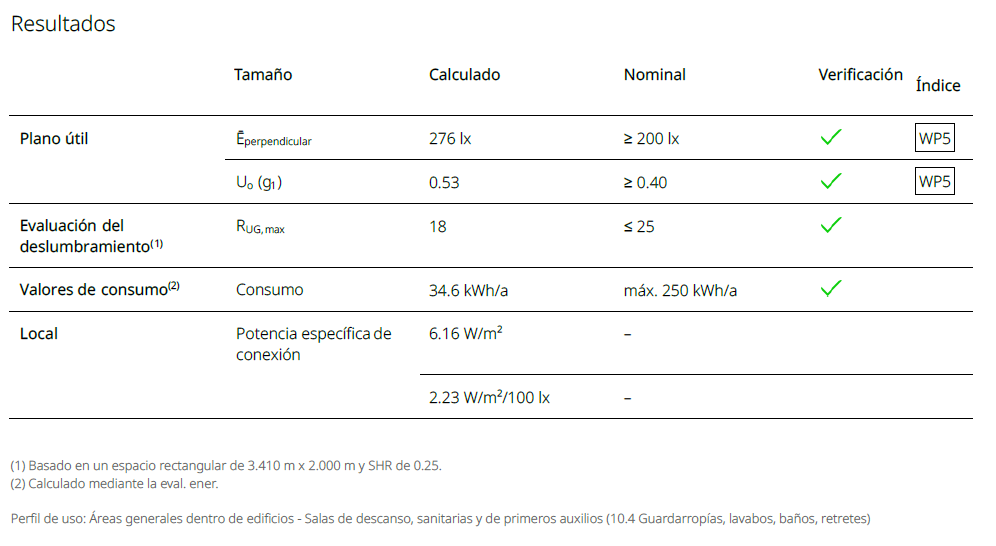
\includegraphics[width=0.75\linewidth]{Imagenes/Resultados Iluminacion Bano Minusvalidos.png}
    \caption{Resultados luminotécnicos Baño Minusválidos.}
\end{figure}

\subsection{Zona Exposición}
\begin{figure}[H]
    \centering
    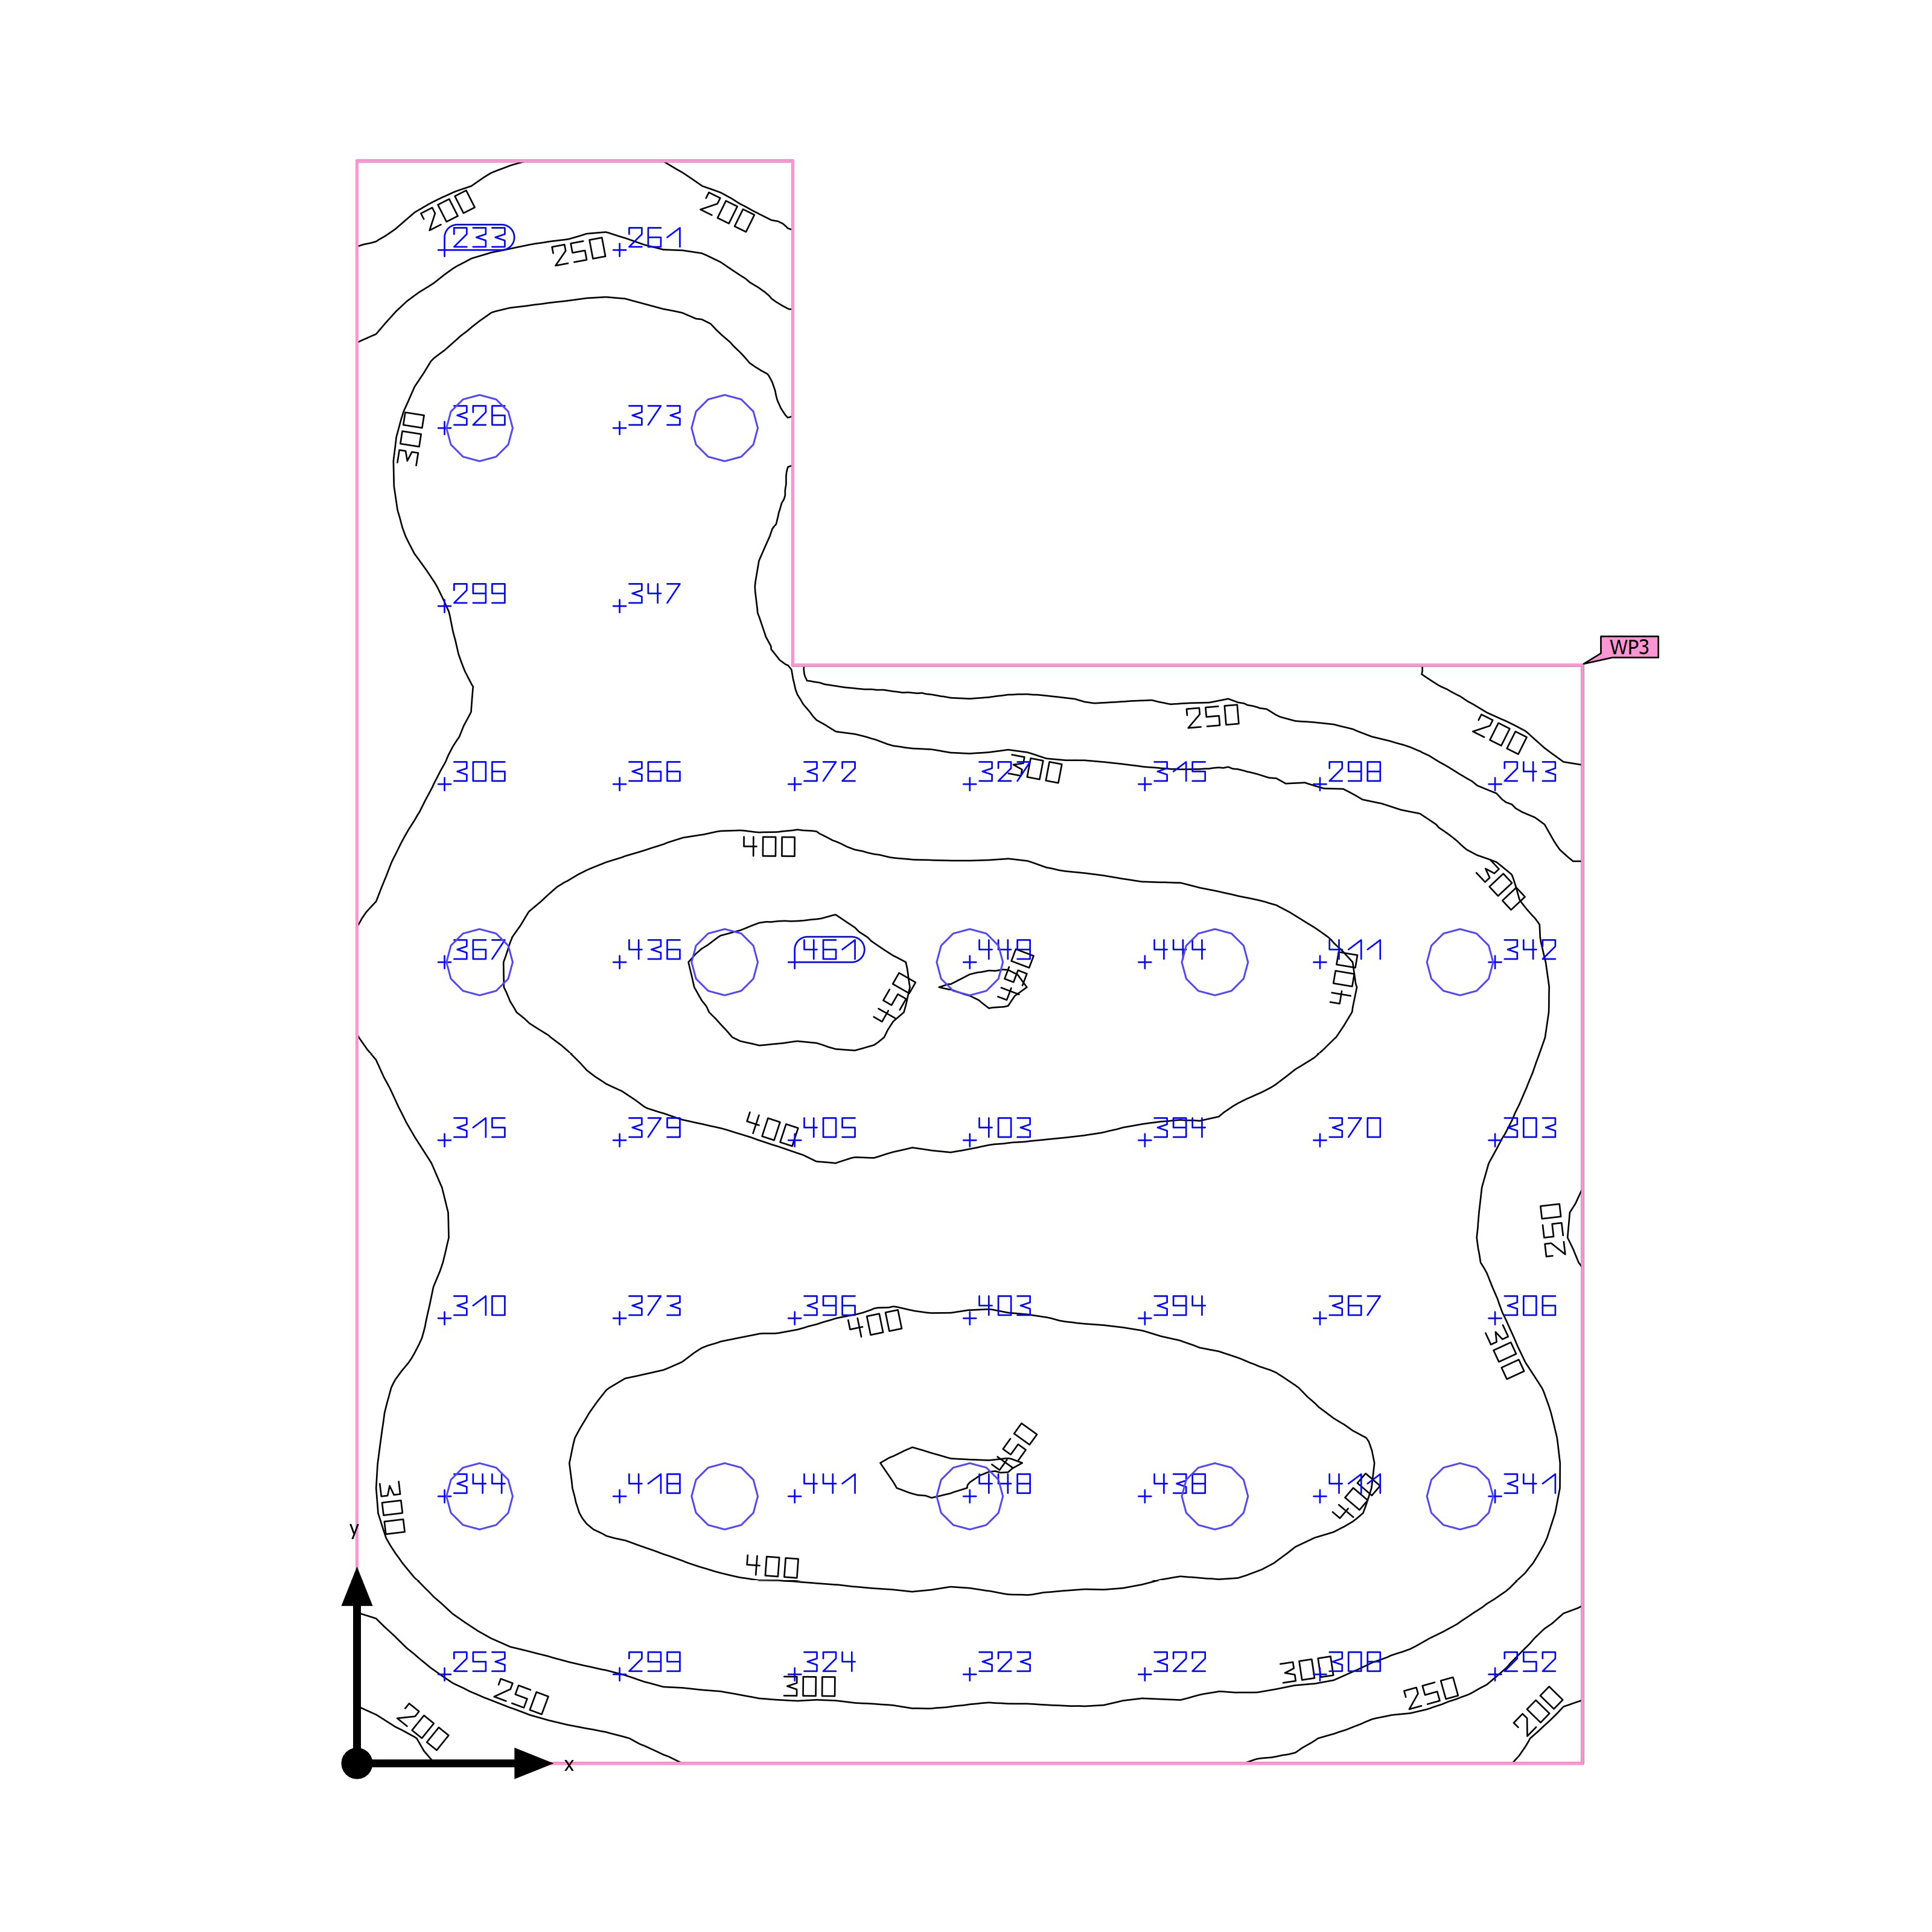
\includegraphics[width=0.5\linewidth]{Imagenes/Iluminacion Zona Exposicion.png}
    \caption{Gráfico flujo luminoso en Zona Exposición.}
\end{figure}

\begin{figure}[H]
    \centering
    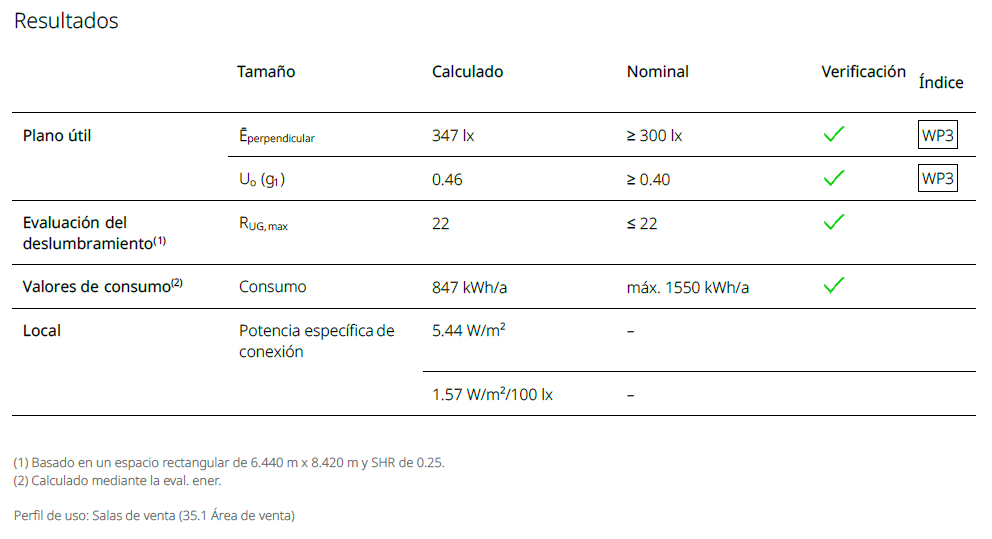
\includegraphics[width=0.75\linewidth]{Imagenes/Resultados Iluminacion Zona Exposicion.png}
    \caption{Resultados luminotécnicos Zona Exposición.}
\end{figure}

\subsection{Oficina}
\begin{figure}[H]
    \centering
    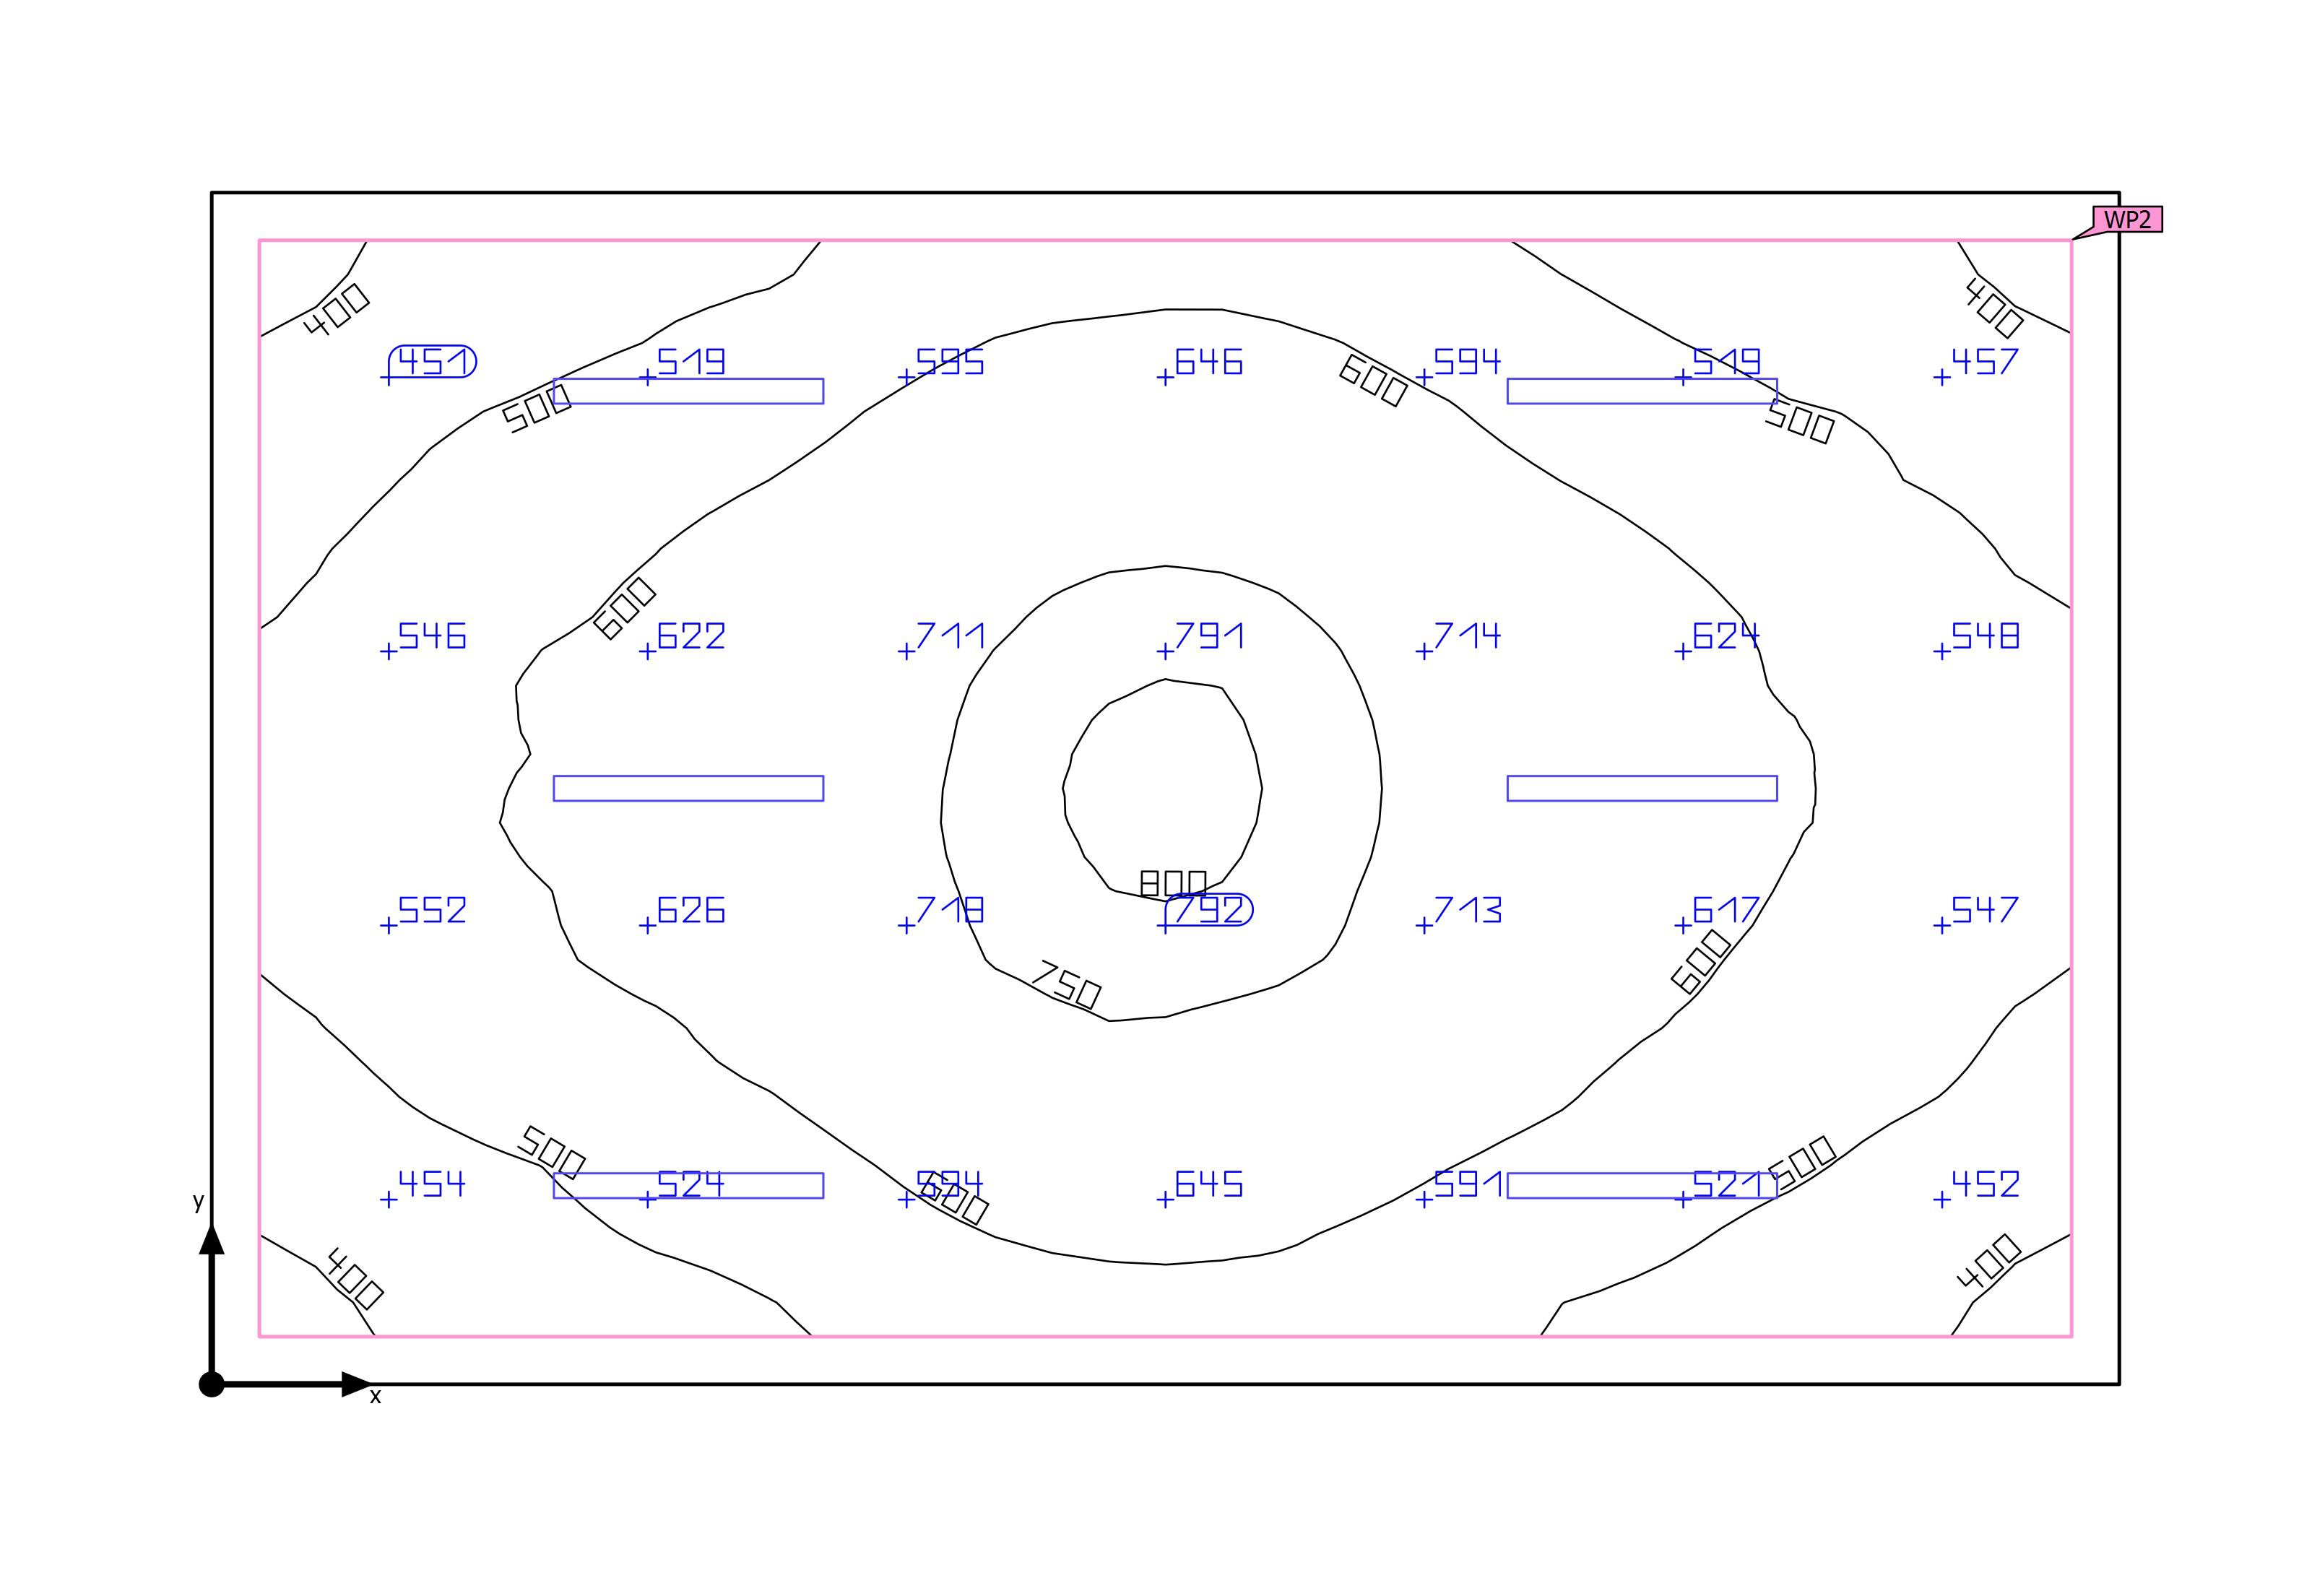
\includegraphics[width=0.5\linewidth]{Imagenes/Iluminacion Oficina.png}
    \caption{Gráfico flujo luminoso en Oficina.}
\end{figure}

\begin{figure}[H]
    \centering
    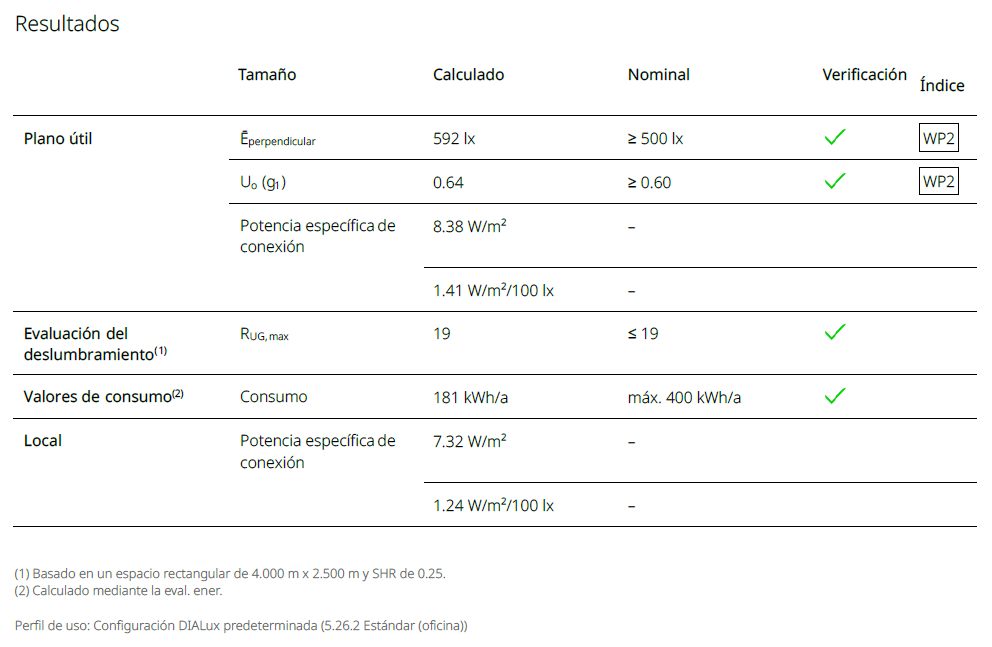
\includegraphics[width=0.75\linewidth]{Imagenes/Resultados Iluminacion Oficina.png}
    \caption{Resultados luminotécnicos Oficina.}
\end{figure}

\subsection{Almacén}
\begin{figure}[H]
    \centering
    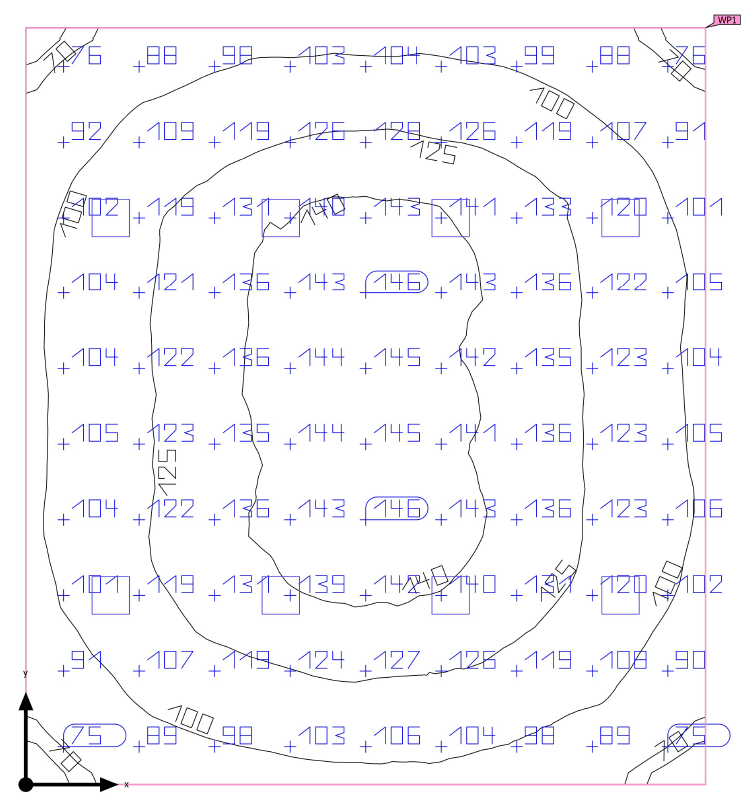
\includegraphics[width=0.5\linewidth]{Imagenes/Iluminacion Almacen.png}
    \caption{Gráfico flujo luminoso en Almacén.}
\end{figure}

\begin{figure}[H]
    \centering
    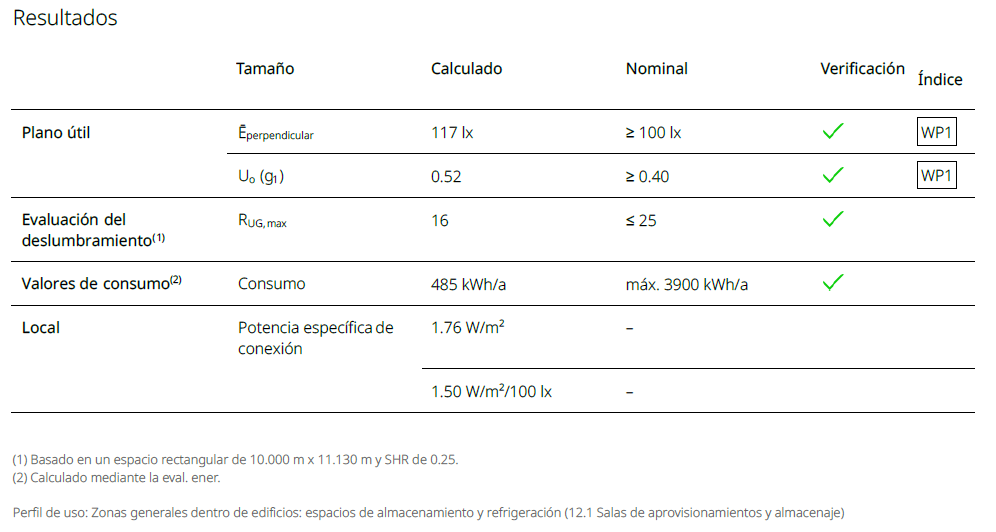
\includegraphics[width=0.75\linewidth]{Imagenes/Resultados Iluminacion Almacen.png}
    \caption{Resultados luminotécnicos Almacén.}
\end{figure}

\subsection{Vestuario Femenino}
\begin{figure}[H]
    \centering
    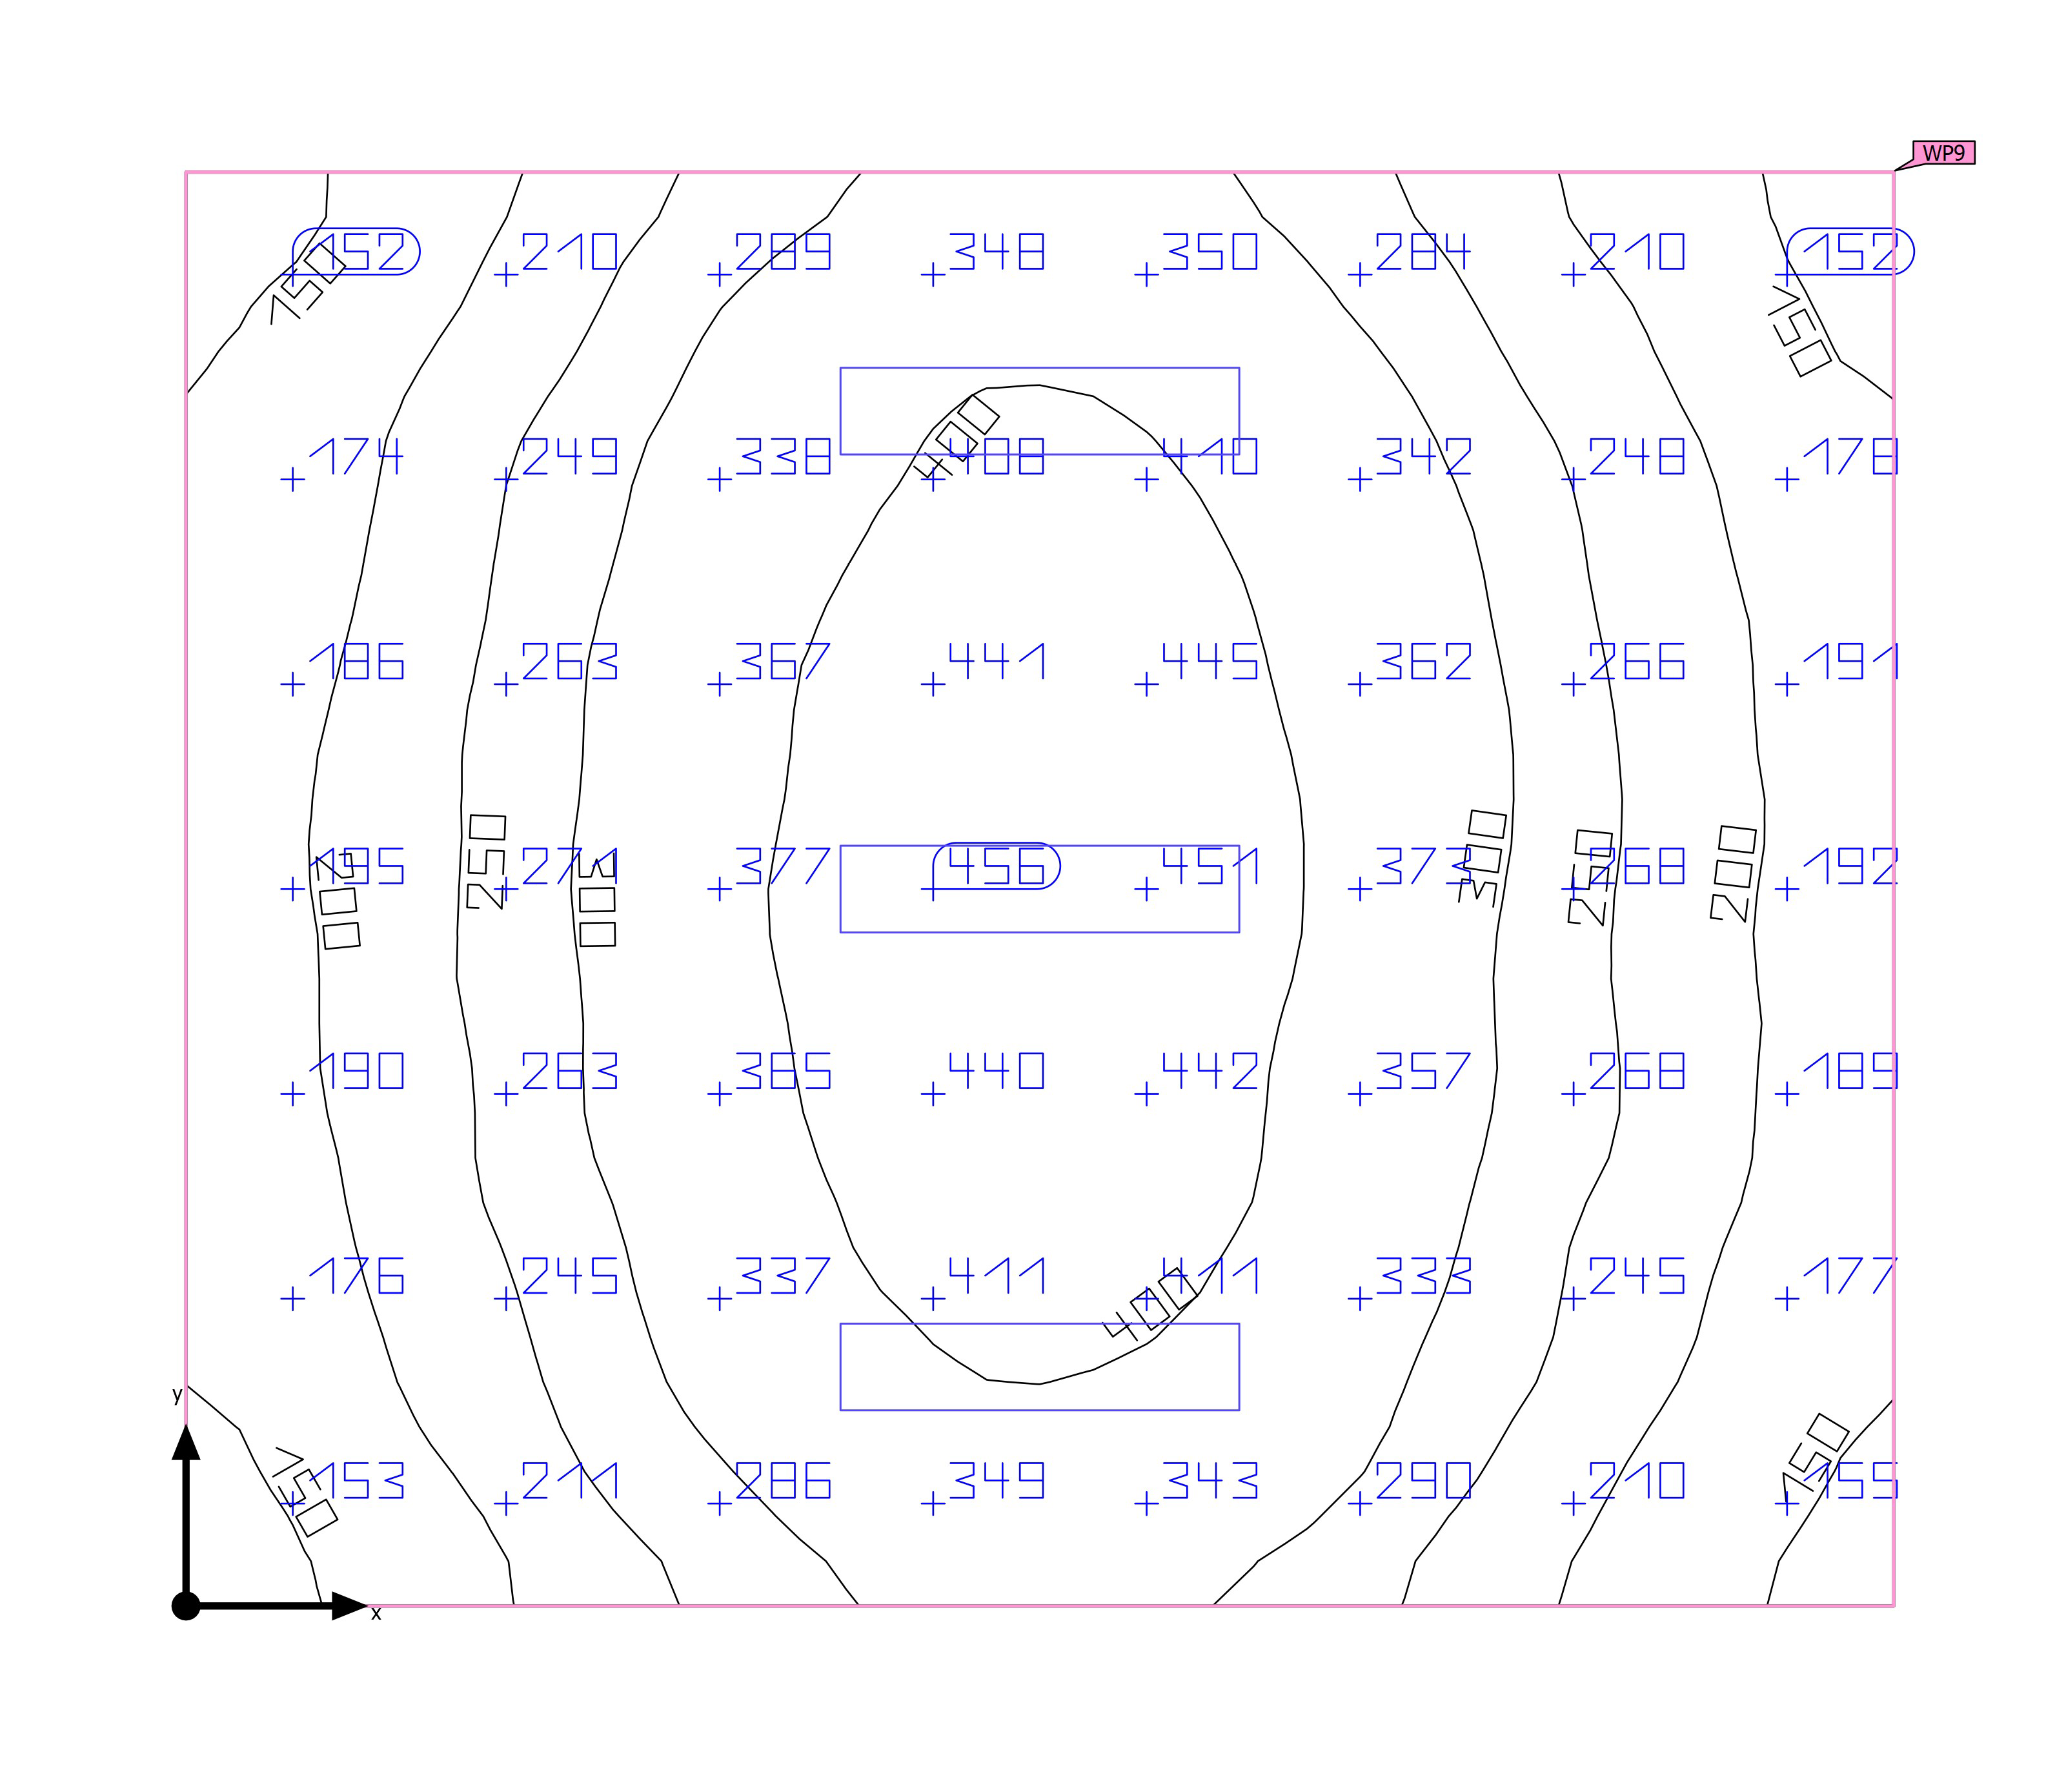
\includegraphics[width=0.5\linewidth]{Imagenes/Iluminacion Vestuario Femenino.png}
    \caption{Gráfico flujo luminoso en Vestuario Femenino.}
\end{figure}

\begin{figure}[H]
    \centering
    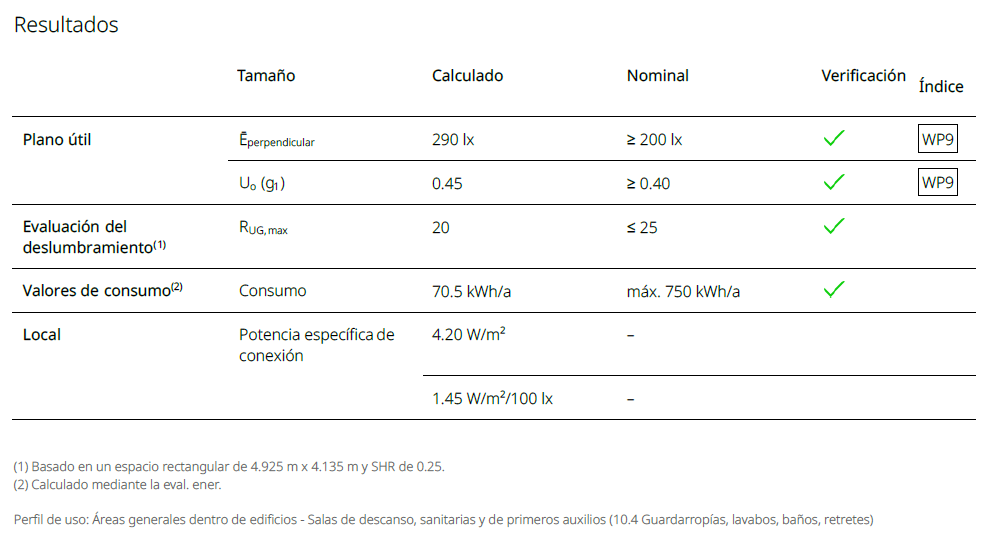
\includegraphics[width=0.75\linewidth]{Imagenes/Resultados Iluminacion Vestuario Femenino.png}
    \caption{Resultados luminotécnicos Vestuario Femenino.}
\end{figure}

\subsection{Vestuario Masculino}
\begin{figure}[H]
    \centering
    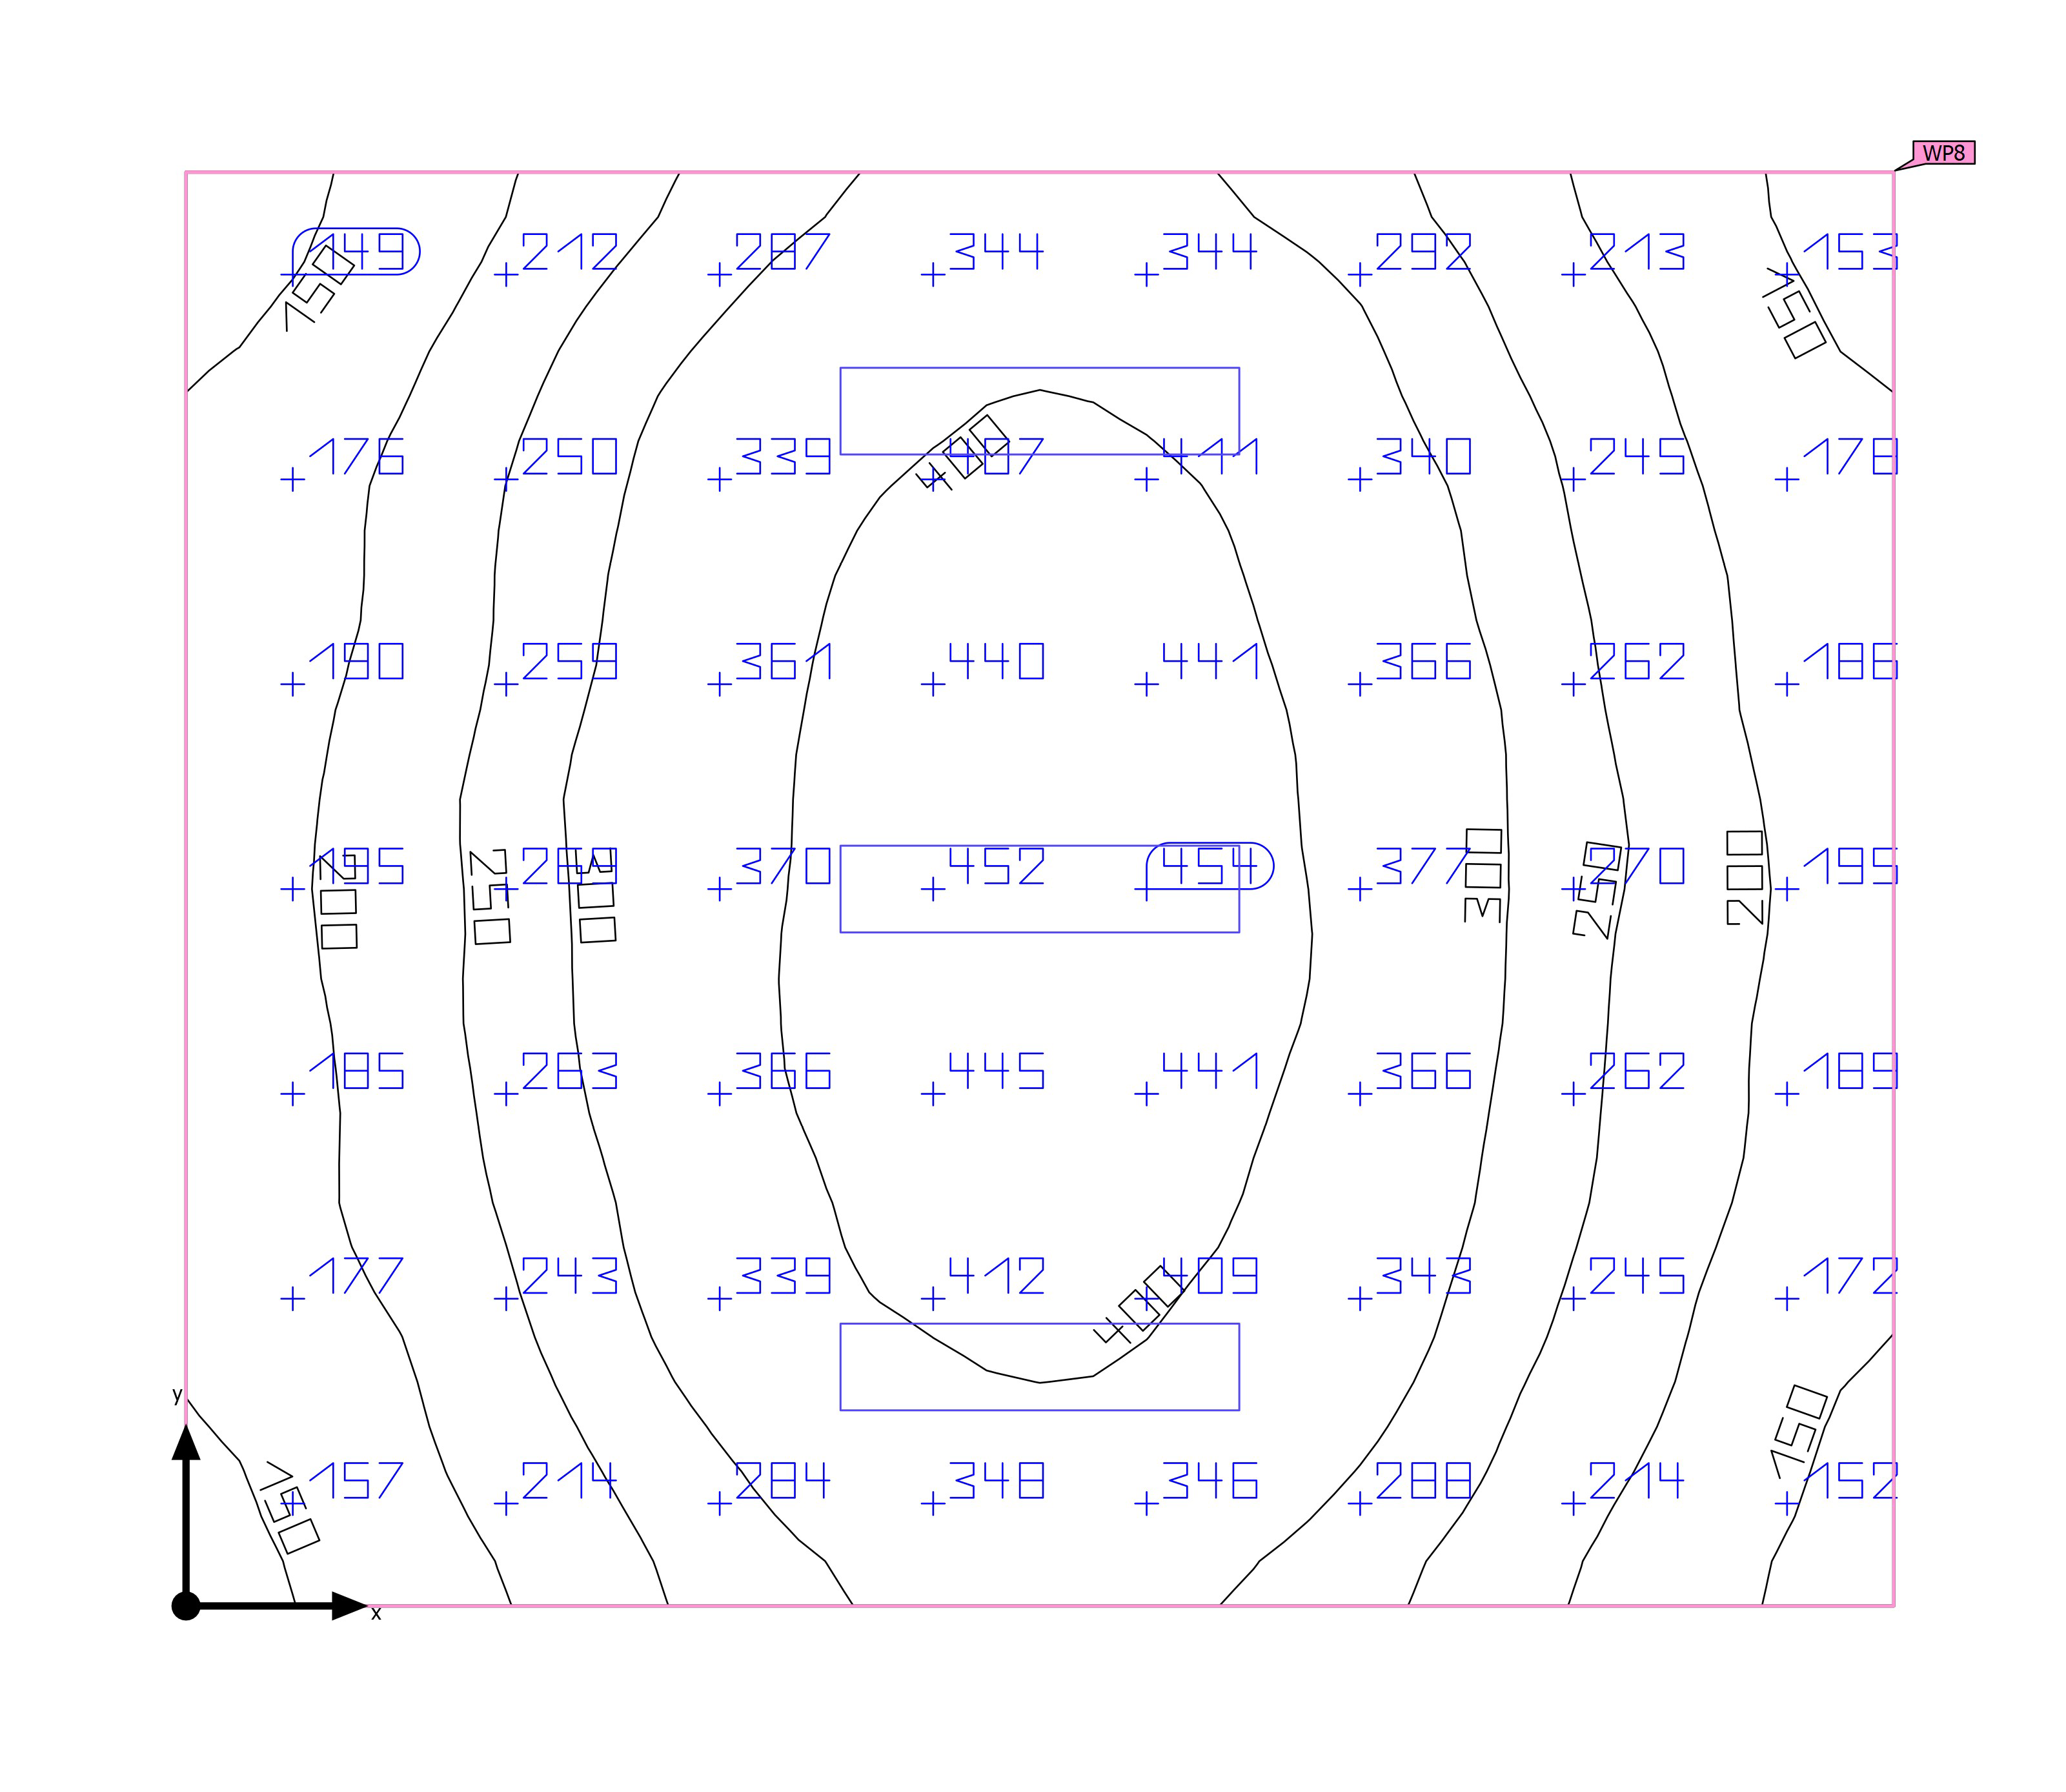
\includegraphics[width=0.5\linewidth]{Imagenes/Iluminacion Vestuario Masculino.png}
    \caption{Gráfico flujo luminoso en Vestuario Masculino.} 
\end{figure}

\begin{figure}[H]
    \centering
    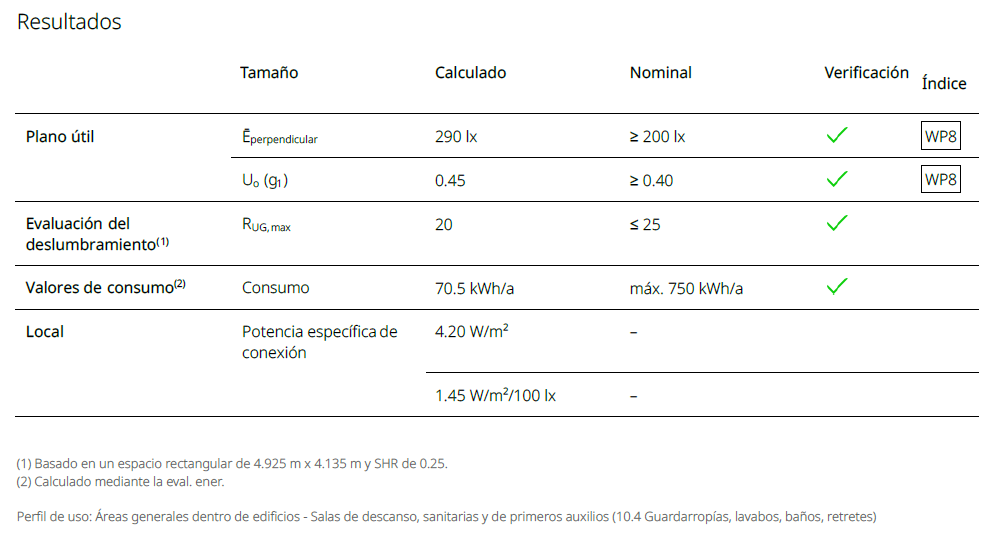
\includegraphics[width=0.75\linewidth]{Imagenes/Resultados Iluminacion Vestuario Masculino.png}
    \caption{Resultados luminotécnicos Vestuario Masculino.}
\end{figure}

\subsection{Zona Descanso}
\begin{figure}[H]
    \centering
    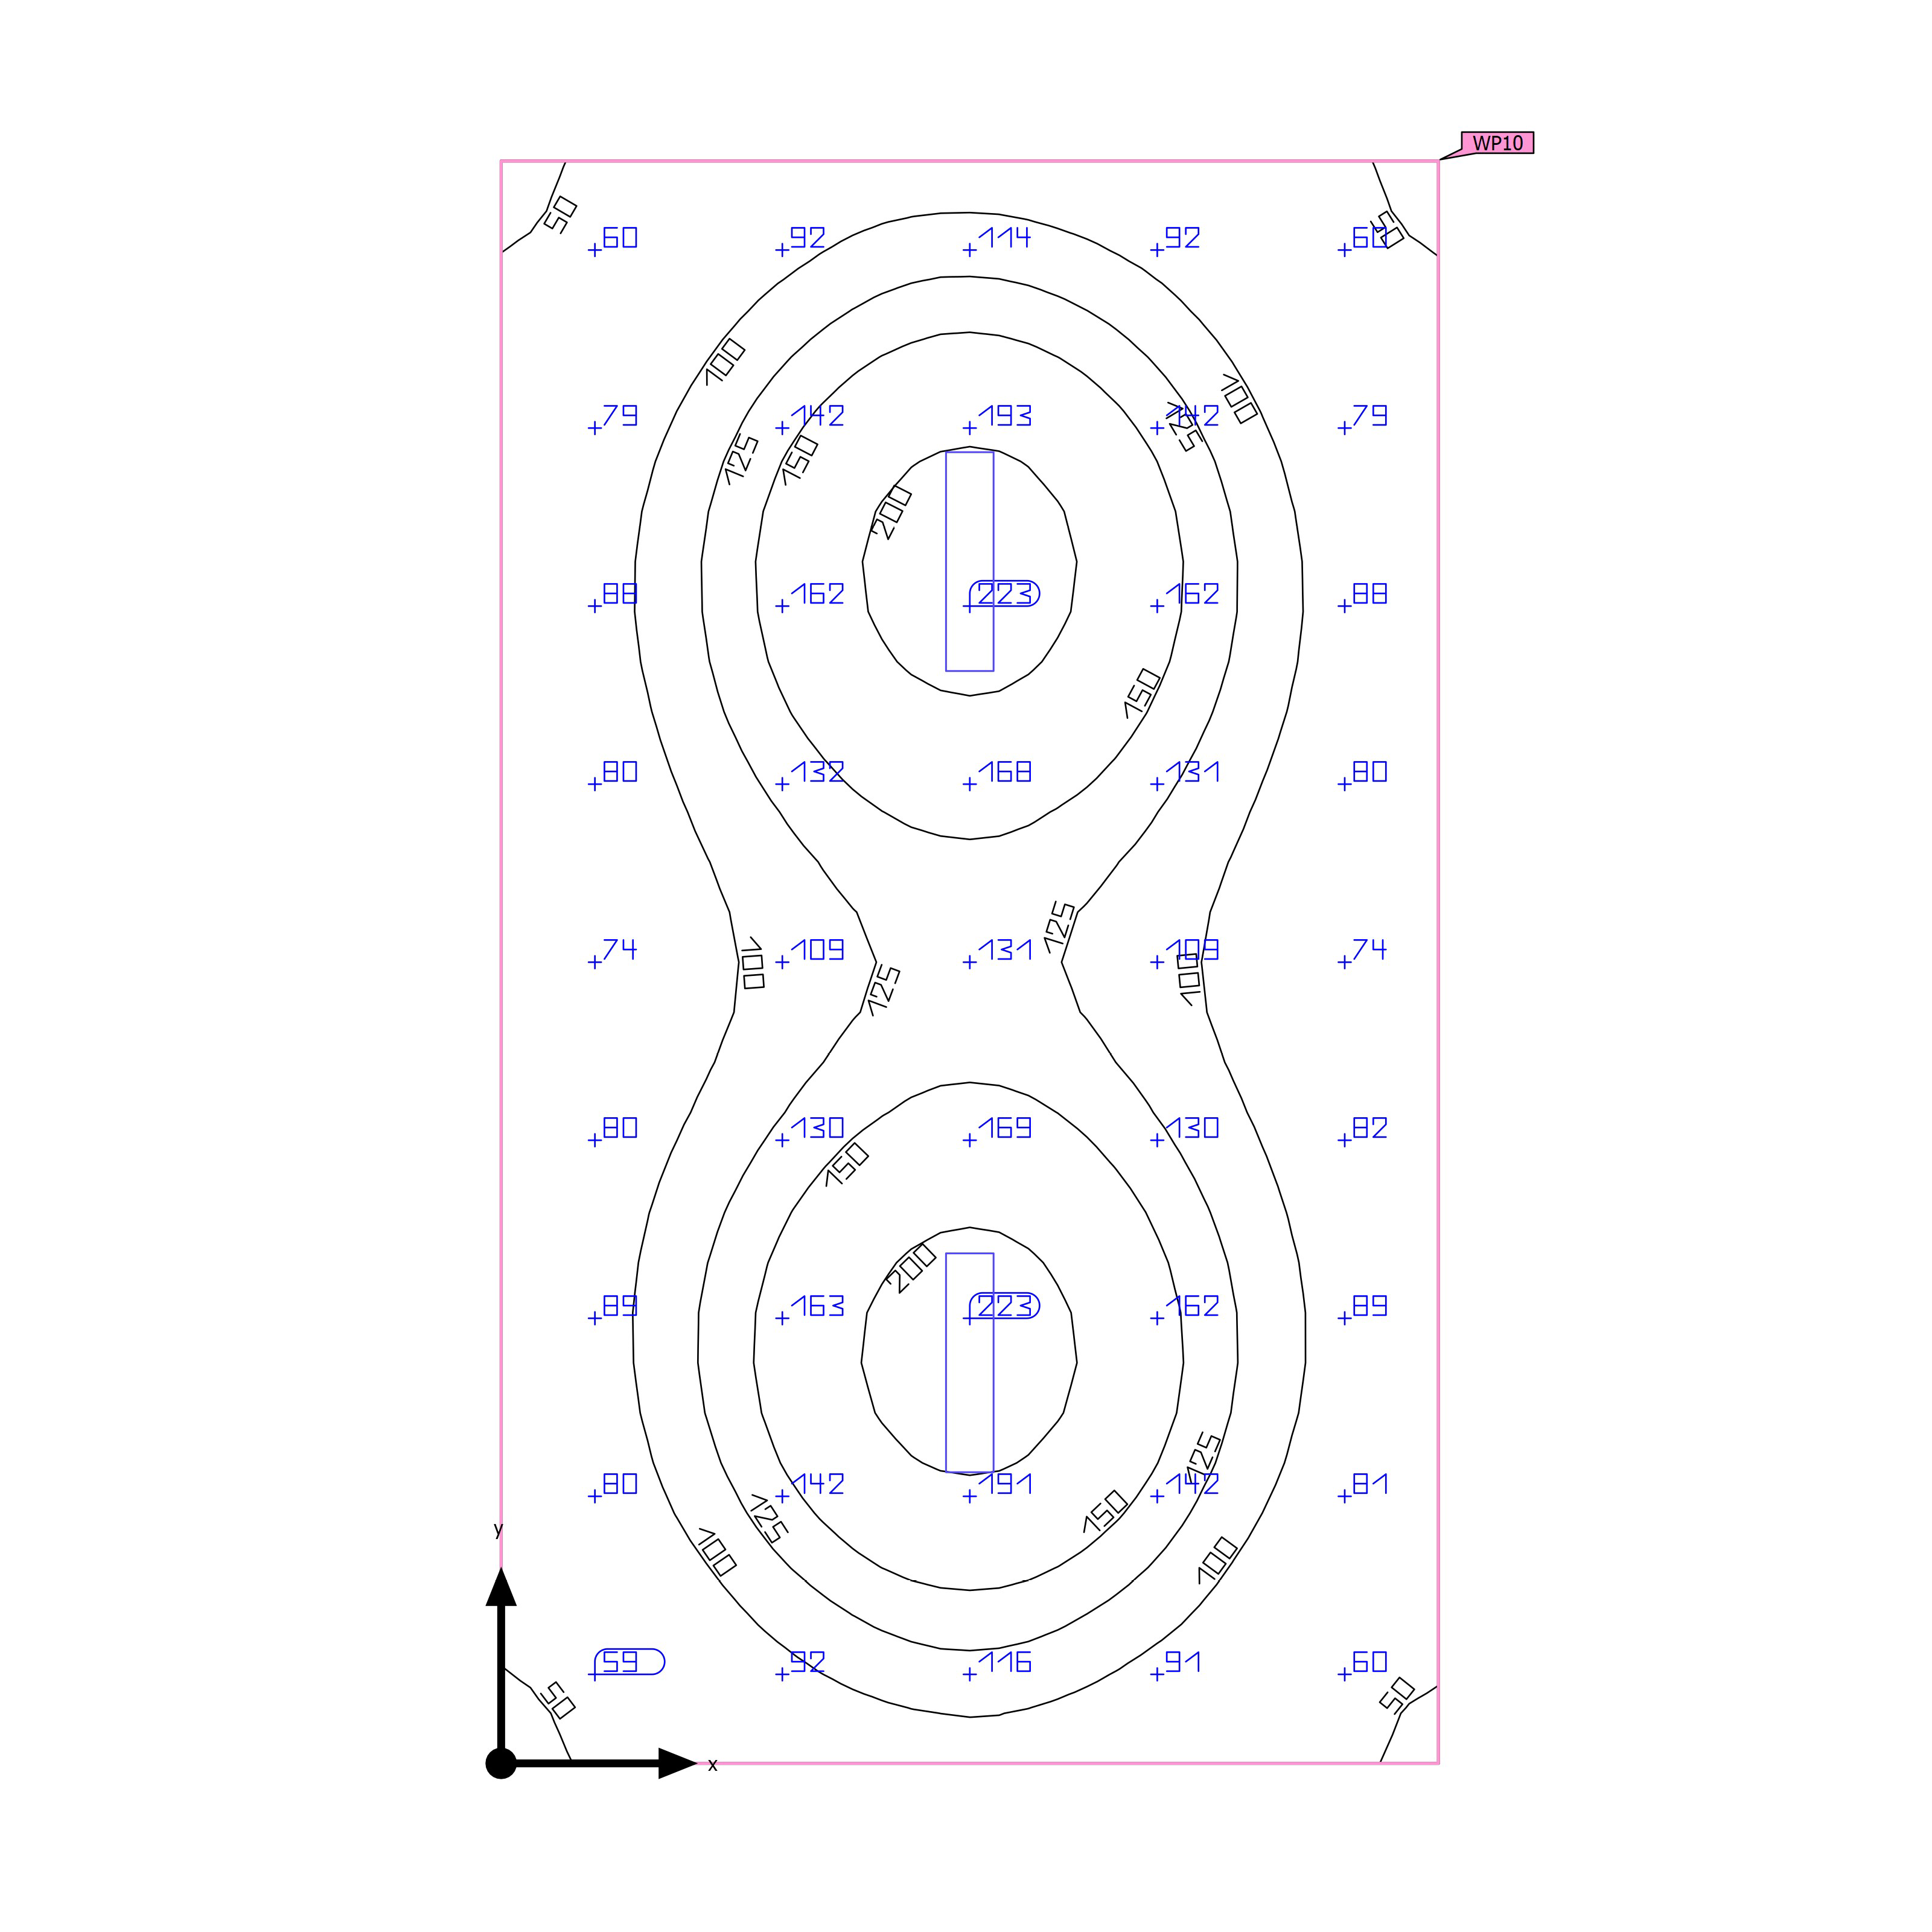
\includegraphics[width=0.5\linewidth]{Imagenes/Iluminacion Zona Descanso.png}
    \caption{Gráfico flujo luminoso en Zona Descanso}
\end{figure}

\begin{figure}[H]
    \centering
    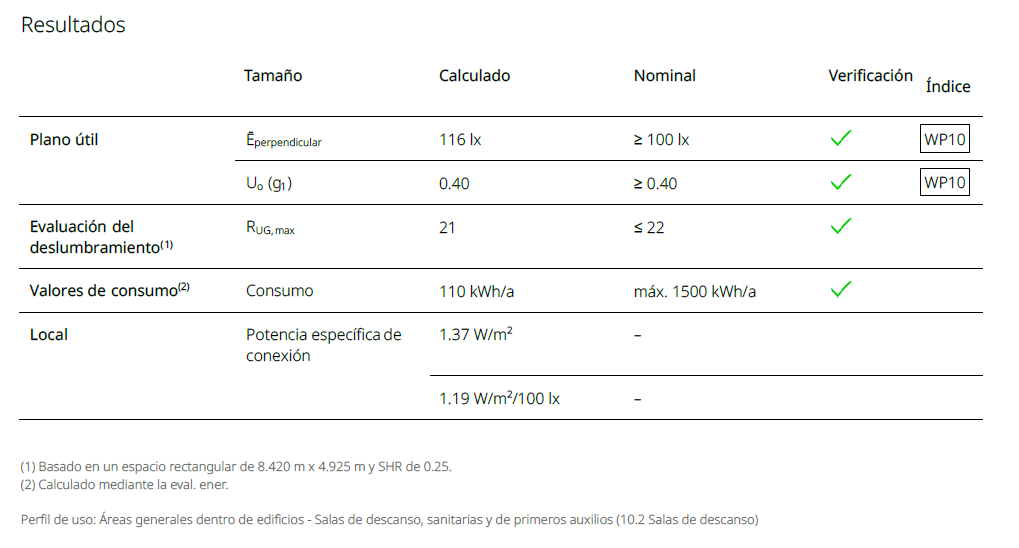
\includegraphics[width=0.75\linewidth]{Imagenes/Resultados Iluminacion Zona Descanso.png}
    \caption{Datos luminotécnicos Zona Descanso.}
\end{figure}

\section{Datos Técnicos de la Luminaria Empleada.}
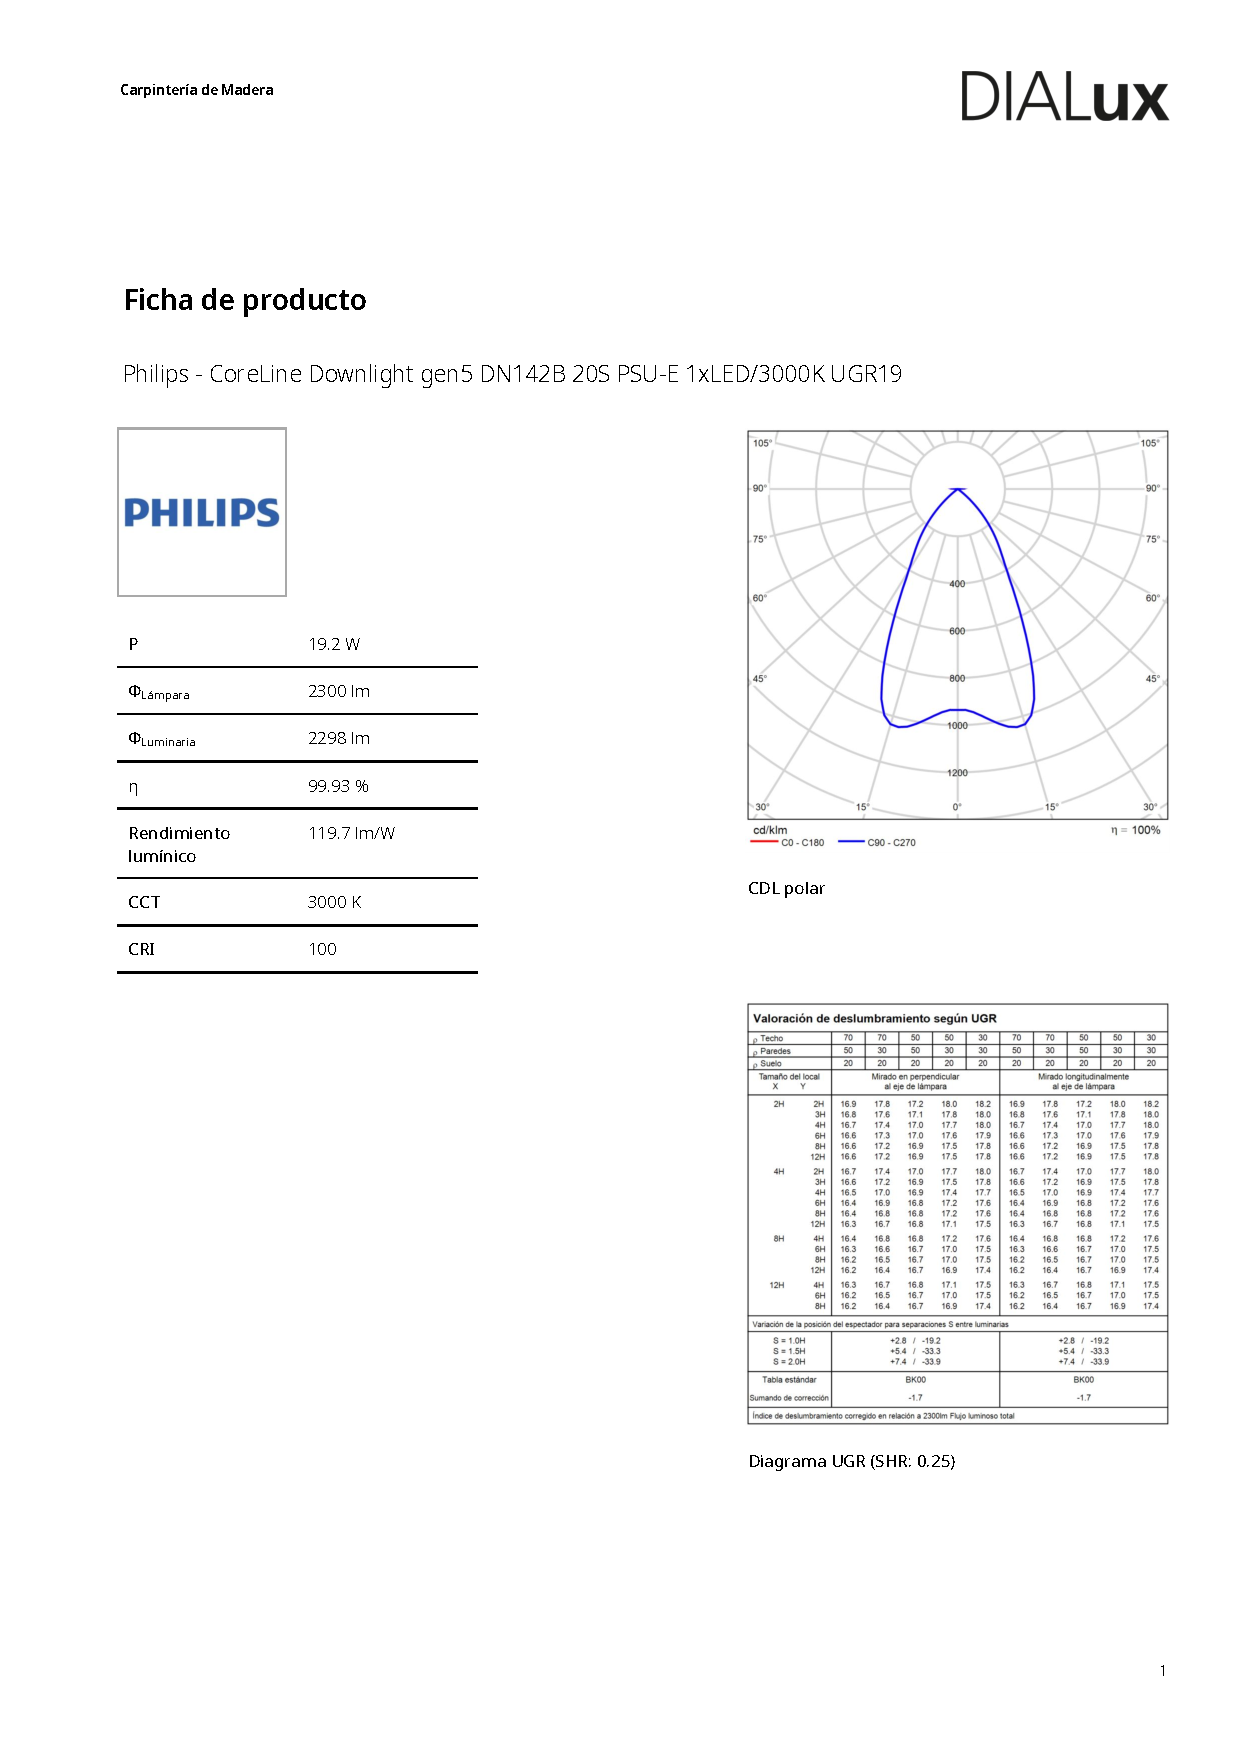
\includepdf[pages={1},pagecommand={
    \thispagestyle{empty}
    \addcontentsline{toc}{subsection}{CoreLine Downlight gen5 DN142B 20S PSU-E 1xLED/3000K UGR19}}]{Otros/Philips - CoreLine Downlight gen5.pdf}

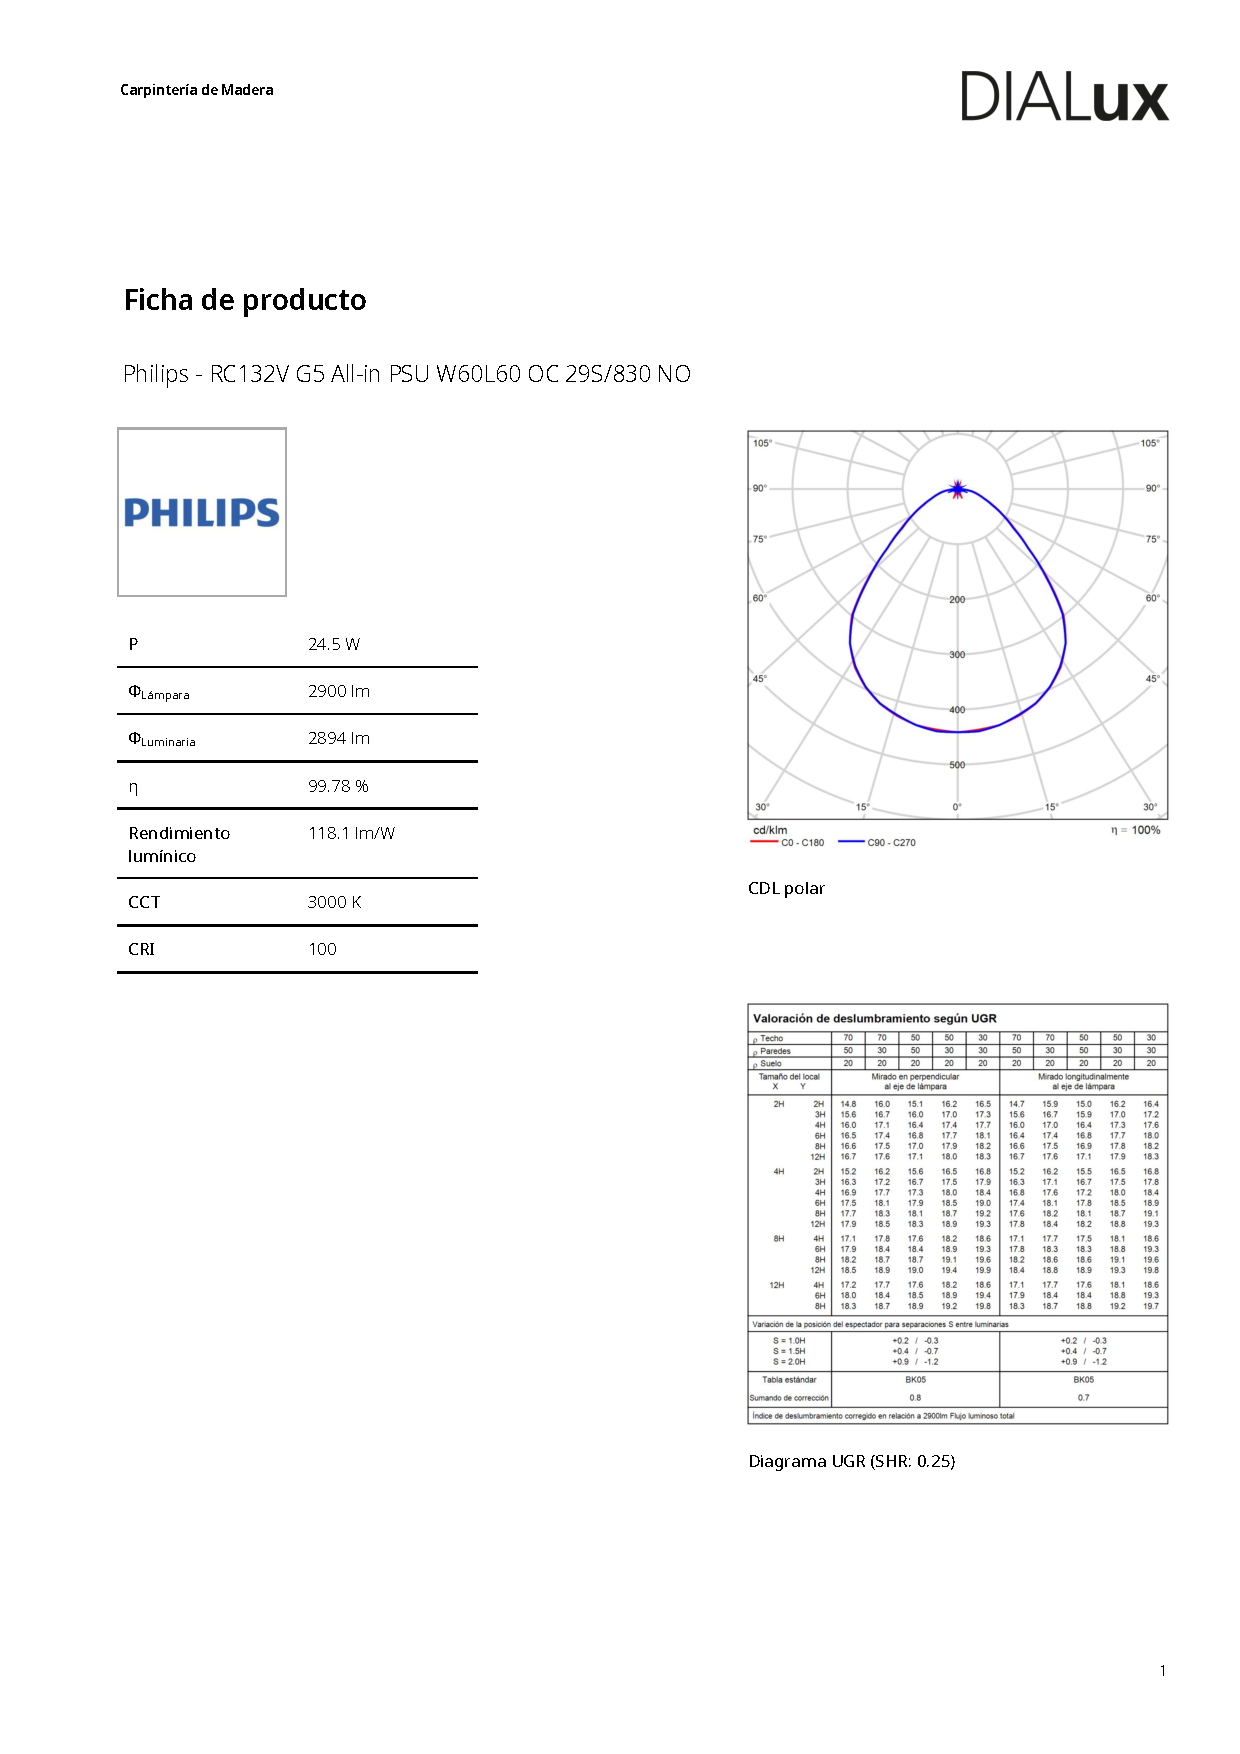
\includepdf[pages={1},pagecommand={
    \thispagestyle{empty}
    \addcontentsline{toc}{subsection}{Philips - RC132V G5 All-in PSU W60L60 OC 29S/830 NO}}]{Otros/Philips - RC132V G5 All-in PSU W60L60.pdf}

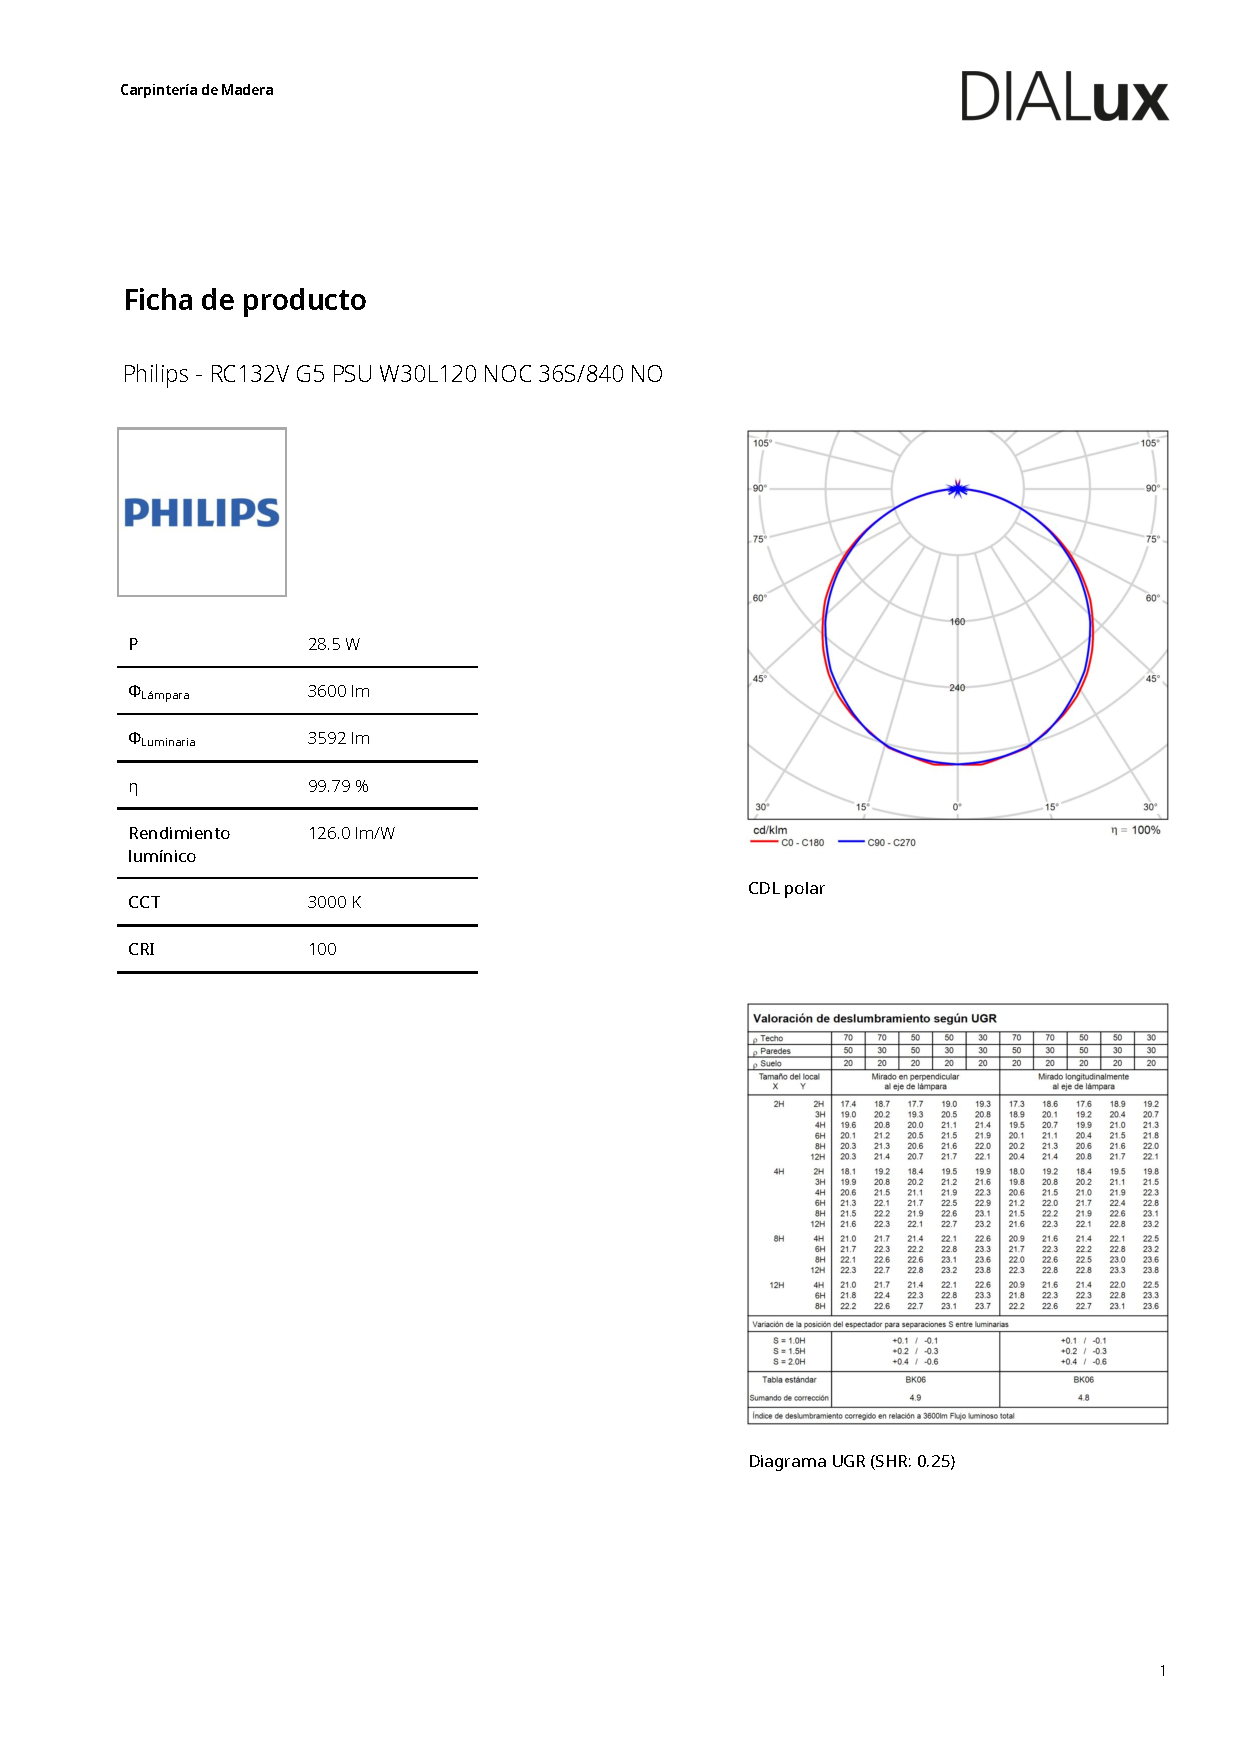
\includepdf[pages={1},pagecommand={
    \thispagestyle{empty}
    \addcontentsline{toc}{subsection}{Philips - RC132V G5 PSU W30L120 NOC 36S/840 NO}}]{Otros/Philips - RC132V G5 PSU W30L120.pdf}

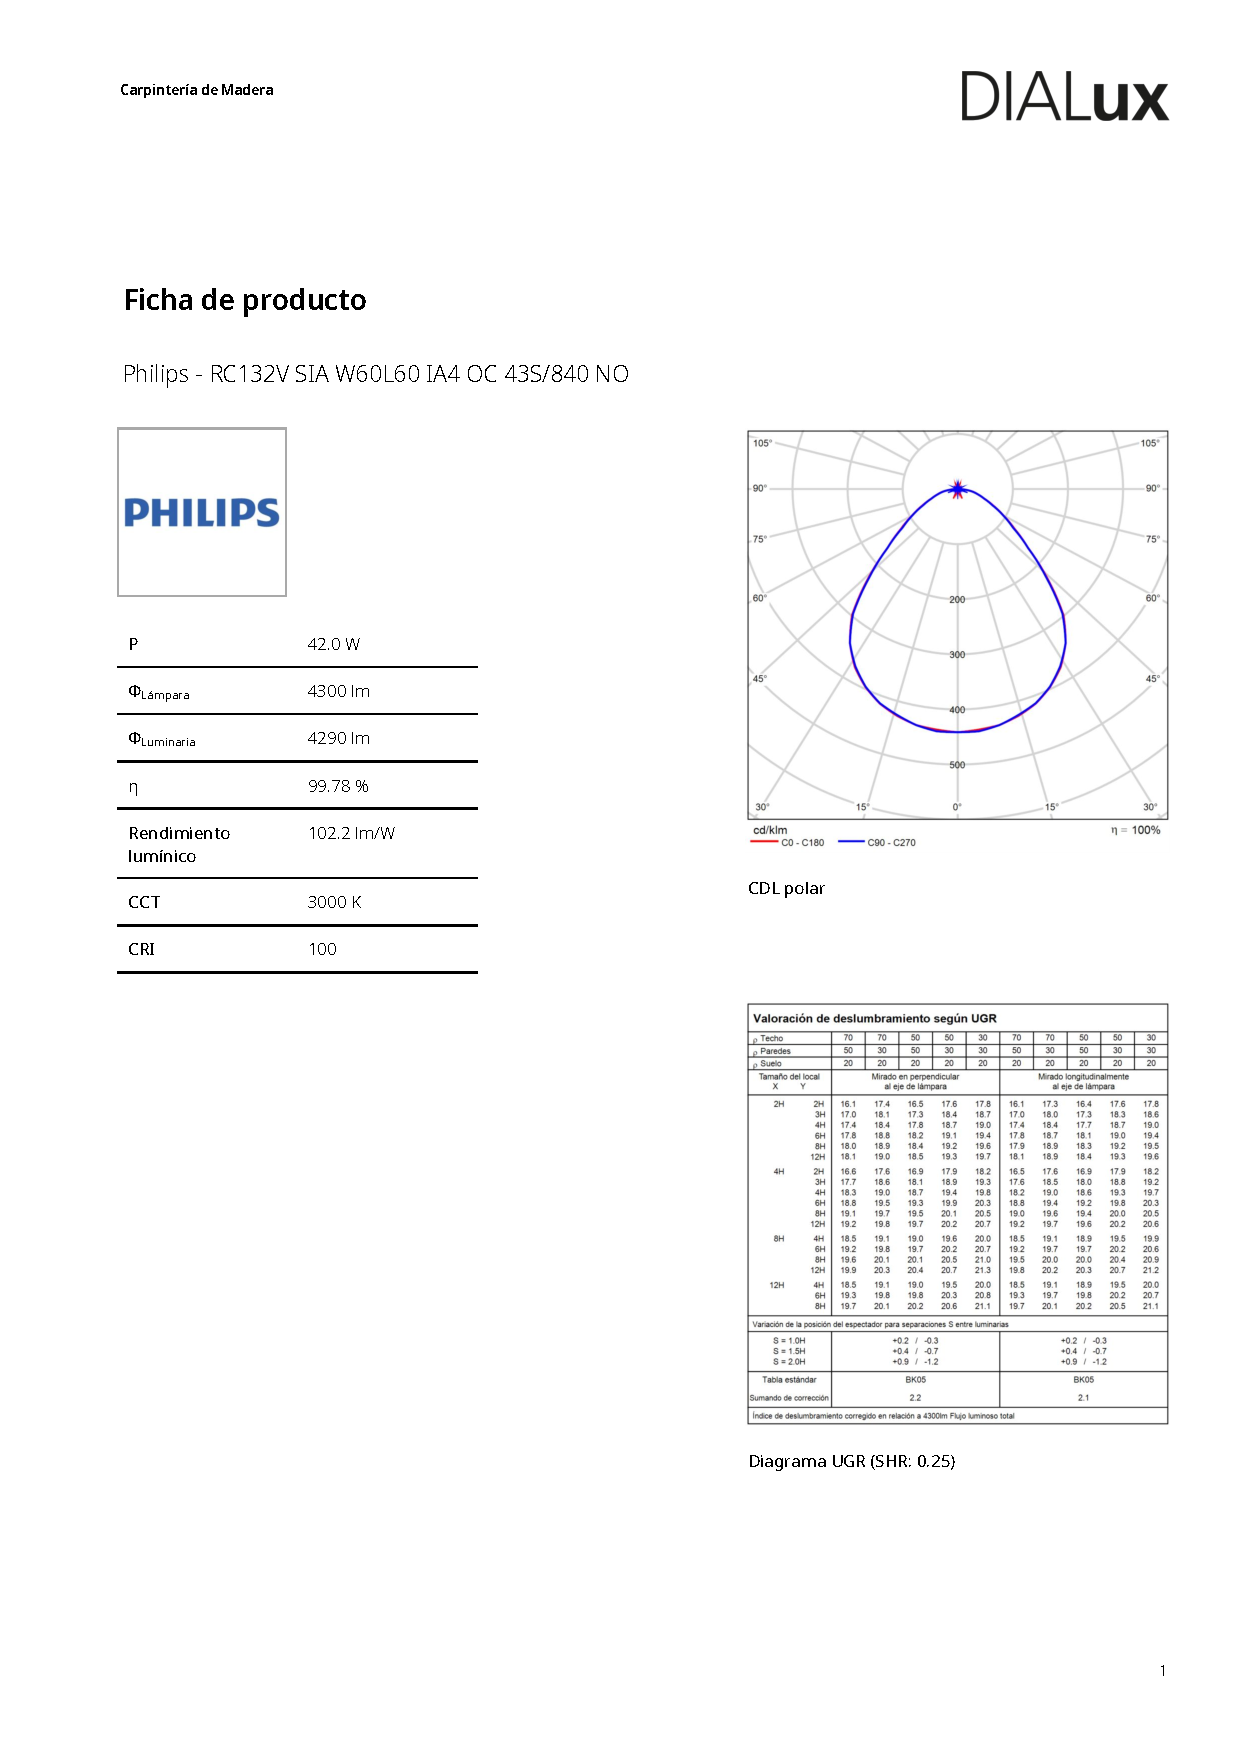
\includepdf[pages={1},pagecommand={
    \thispagestyle{empty}
    \addcontentsline{toc}{subsection}{Philips - RC132V SIA W60L60 IA4 OC 43S/840 NO}}]{Otros/Philips - RC132V SIA W60L60.pdf}

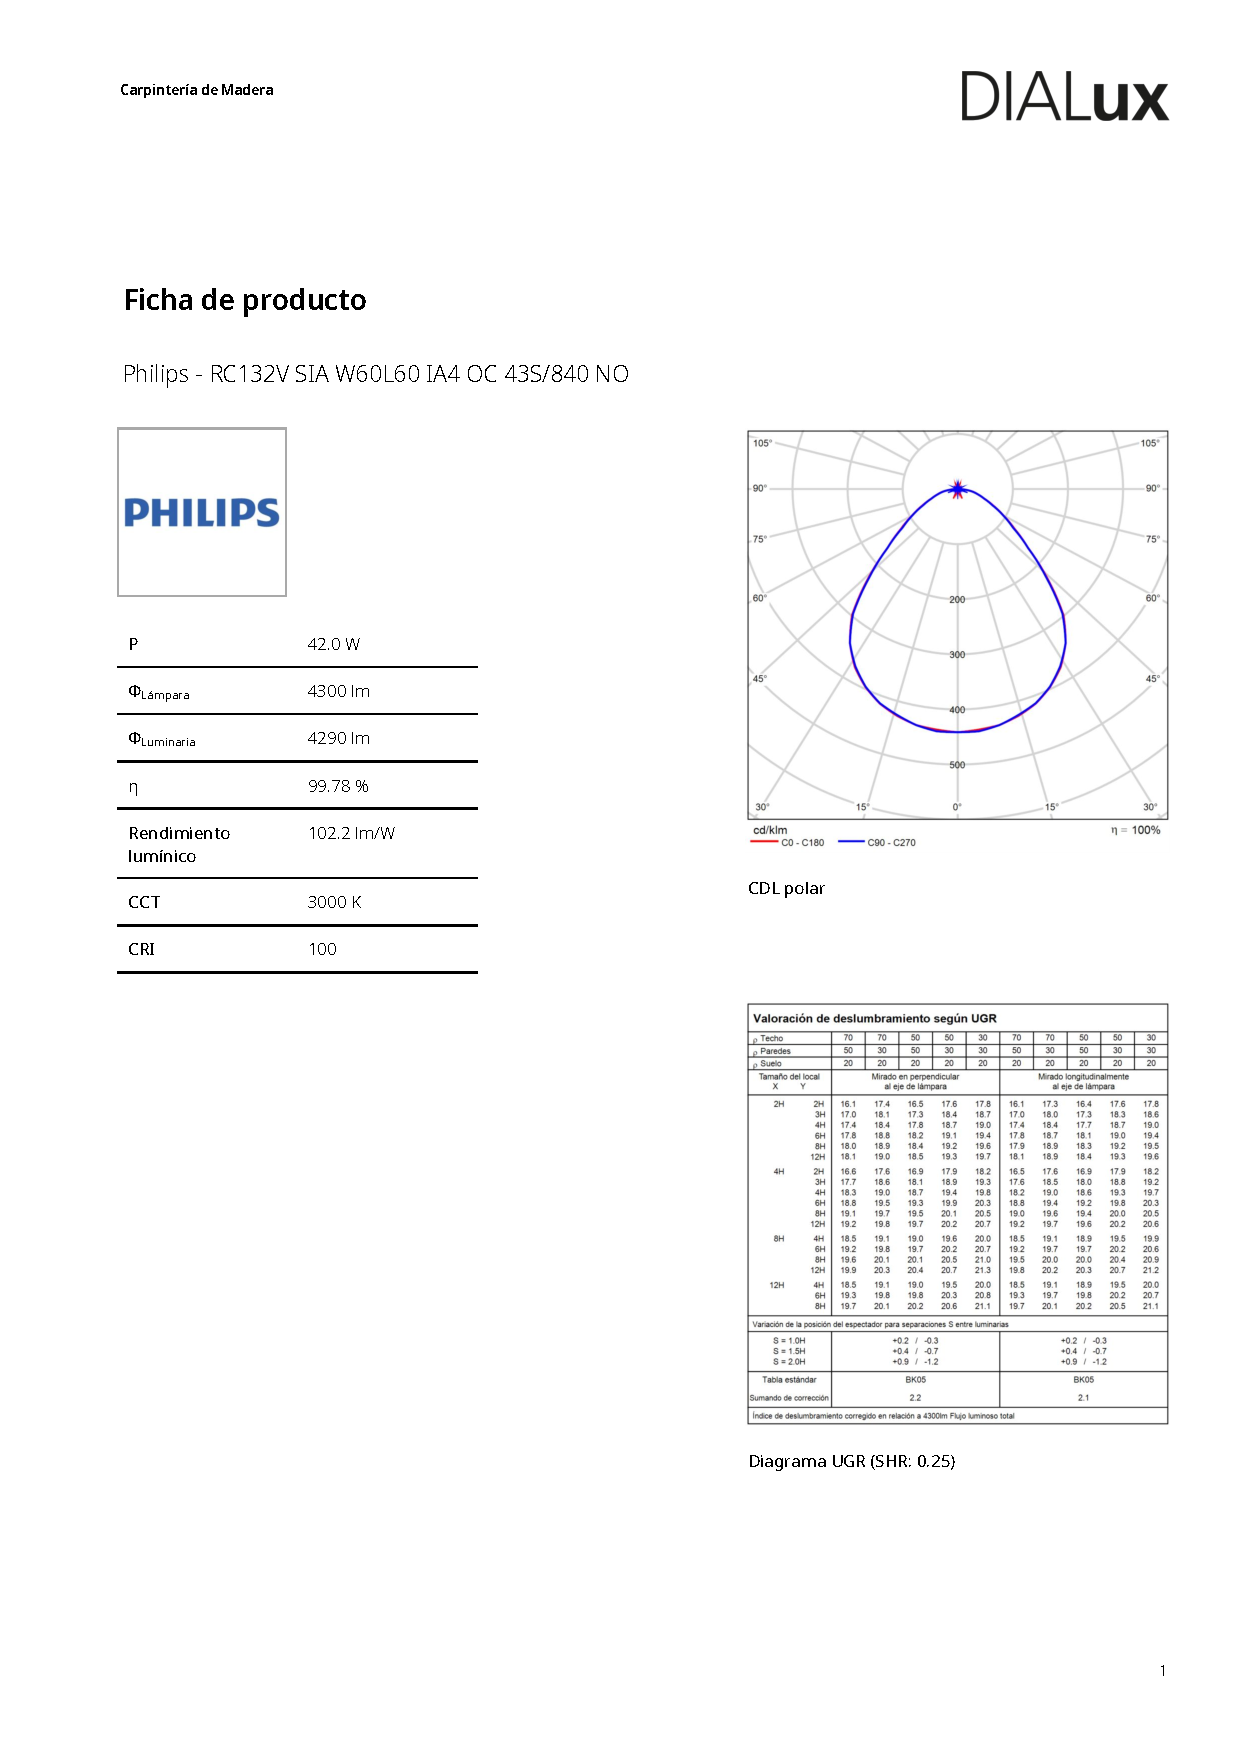
\includepdf[pages={1},pagecommand={
    \thispagestyle{empty}
    \addcontentsline{toc}{subsection}{Philips - SP530P PSD L570 OC LED17S/940 NO}}]{Otros/Philips - RC132V SIA W60L60.pdf}

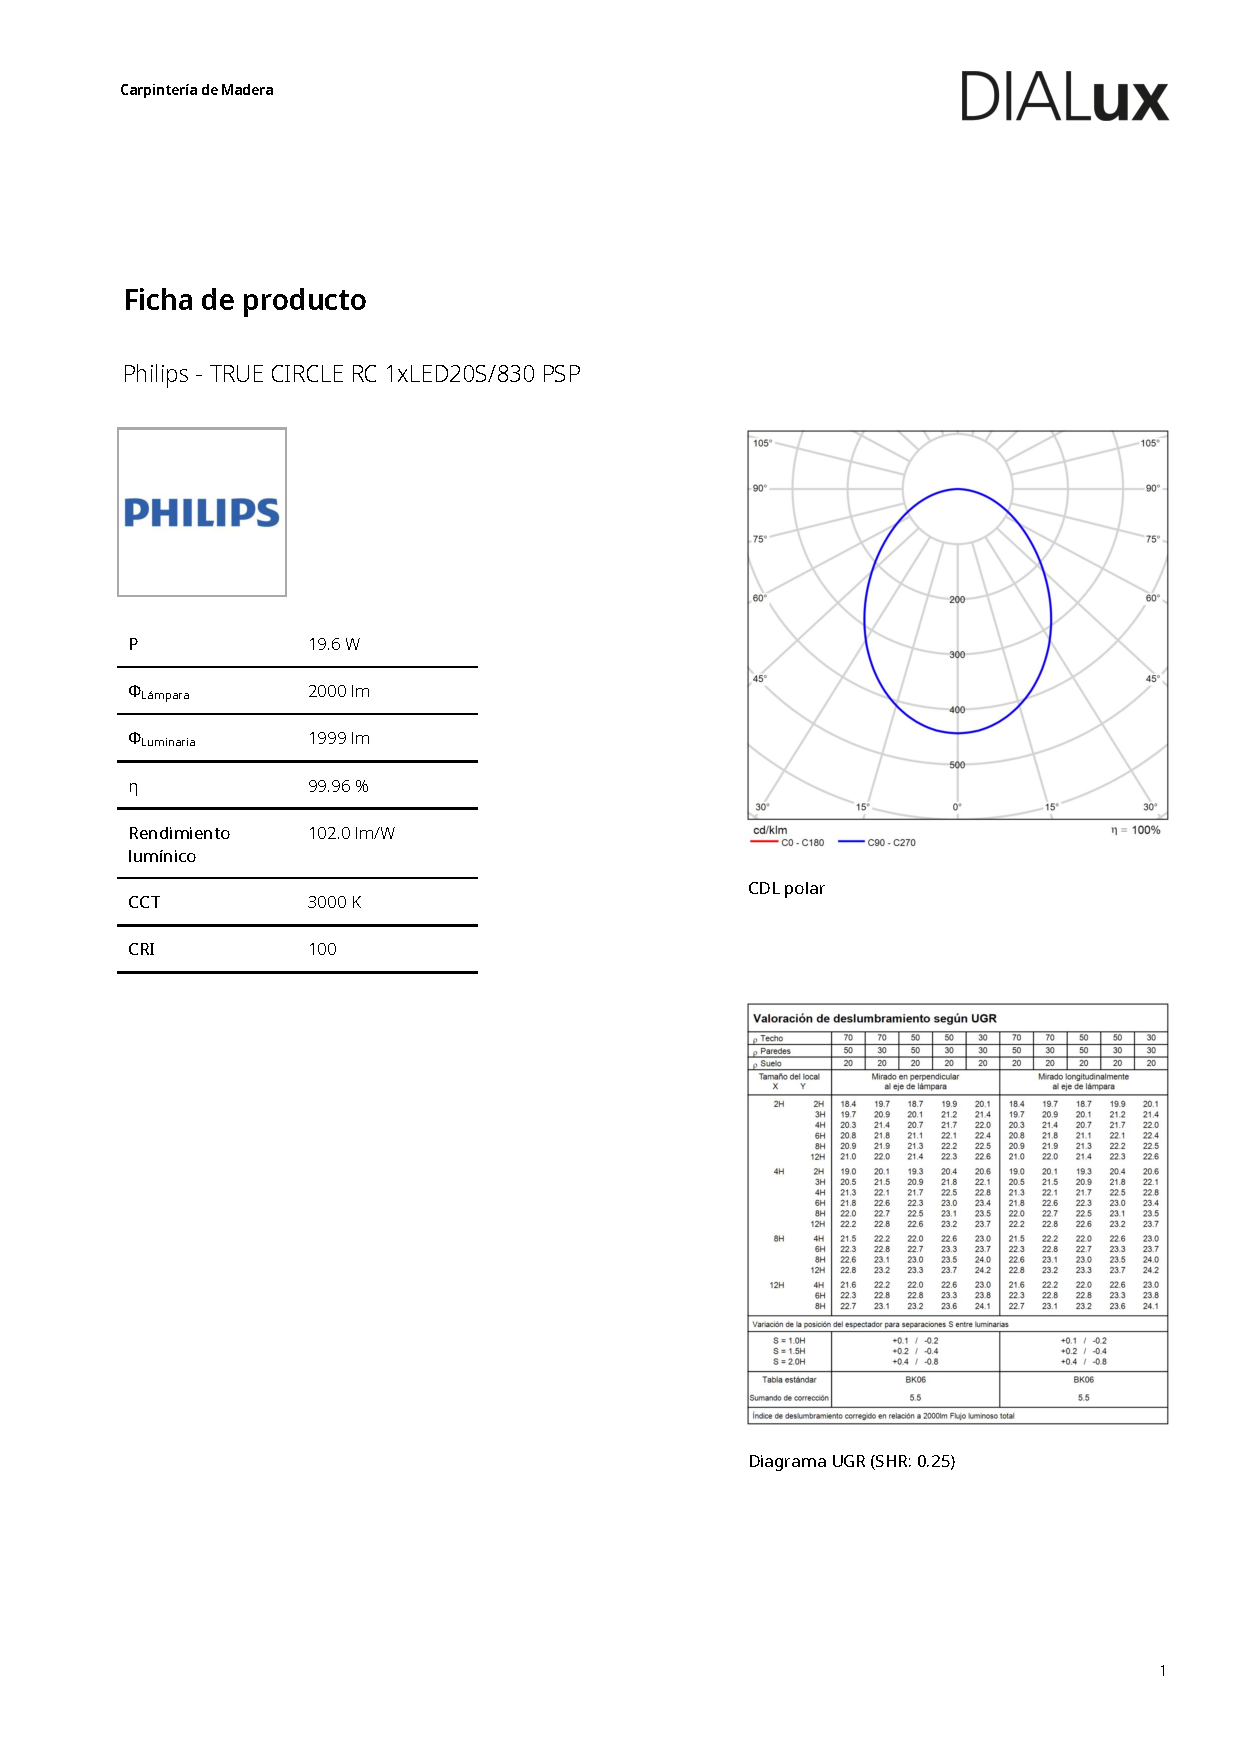
\includepdf[pages={1},pagecommand={
    \thispagestyle{empty}
    \addcontentsline{toc}{subsection}{Philips - TRUE CIRCLE RC 1xLED20S/830 PSP}}]{Otros/Philips - TRUE CIRCLE.pdf}
    
\end{document}